\chapter{Wiadukt WK2 w ciągu Pomorskiej Kolei Metropolitalnej}

\section{Charakterystyka obiektu}
Obiekt badawczy stanowi kolejowy wiadukt łukowy w ciągu linii Pomorskiej Kolei Metropolitalnej w km 1+696,02. Przęsło wiaduktu stanowi stalowy ustój łukowy z jazdą dołem. Widok z boku na konstrukcję stalową wiaduktu pokazano na rysunkach \ref{fig: wk2_side_view}. Główne wymiary charakteryzujące konstrukcję to: 
\begin{itemize}[noitemsep]
	\item rozpiętość teoretyczna: $L_t=70.00 \text{m}$, 
	\item długość całkowita:  $L_c=71,60 \text{m}$, 
	\item wysokość w kluczu:  $H=11.00 \text{m}$,
	\item rozstaw osiowy dźwigarów: $B_t = 7.35 \text{m}$,
	\item szerokość całkowita: $B_c=10.21 \text{m}$. 
\end{itemize}
 \begin{figure}[h]
	\centering
	\subfloat{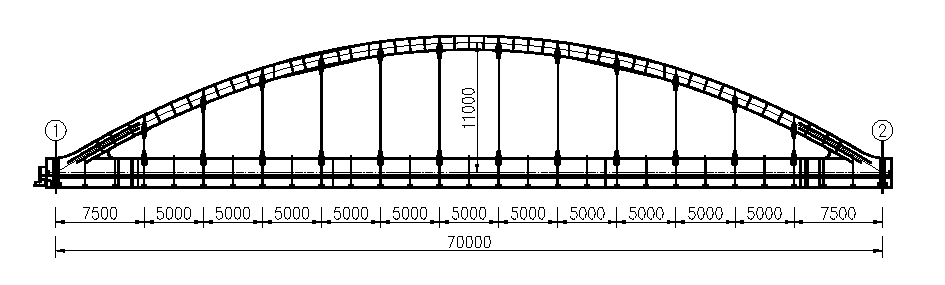
\includegraphics{/WK2/rysunki/widok_z_boku_croped.pdf}} 
	\captionsetup{justification=centering}
	\caption{Widok z boku na konstrukcję stalową dźwigara łukowego wiaduktu WK3}
	\label{fig: wk2_side_view}
\end{figure}

 Przekrój poprzeczny dźwigarów łukowych zaprojektowano jako skrzynkowy (rys. \ref{fig: wk2_cross_sect}). Pomost wykonano jako ortotropowy, z blachy wzmocnionej żebrami podłużnymi i poprzecznicami o przekroju teowym. Poprzecznice rozmieszczono w rozstawie 2.5 m. Ściąg łuku stanowią belki dwuteowe, po jednej dla każdego dźwigara łukowego. Przekrój ściągu zmienia się z dwuteowego na skrzynkowy w strefie podporowej. Na rysunku \ref{fig: wk2_cross_sect_deck} przestawiono przekrój poprzeczny pomostu i ściągu w strefie podporowej. 
  \begin{figure}[h]
 	\centering
 	\subfloat{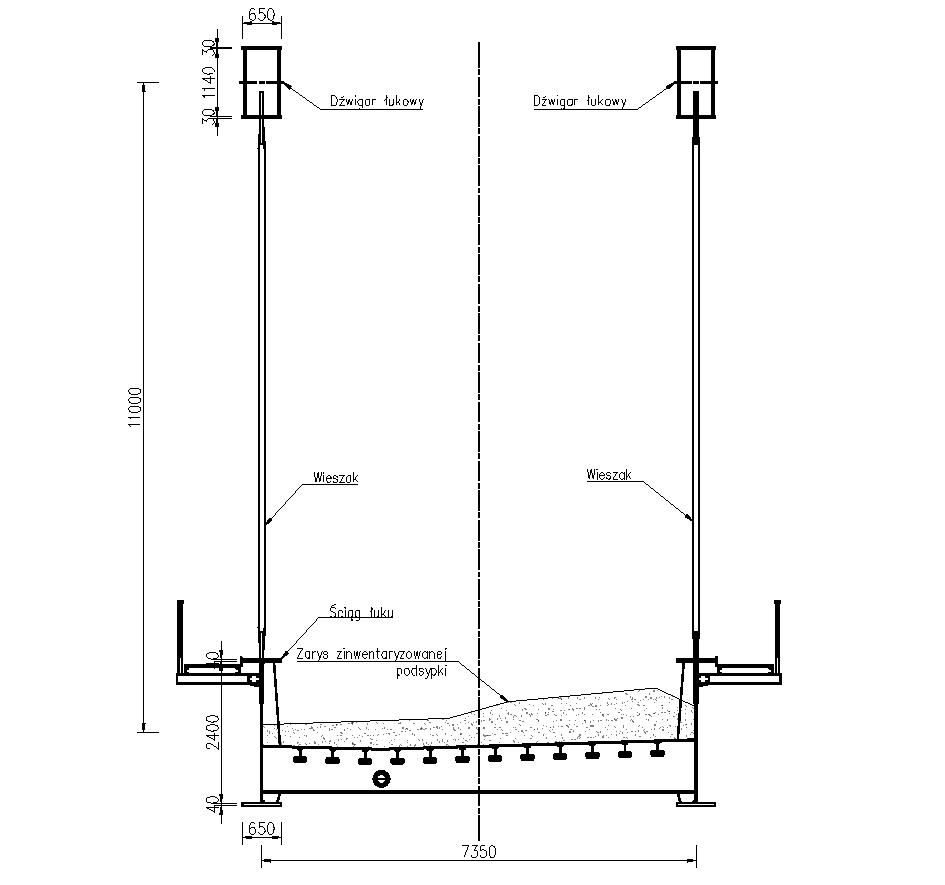
\includegraphics[height=0.6\textheight]{/WK2/rysunki/przekroj_dzwigara_croped.pdf}} 
 	\captionsetup{justification=centering}
 	\caption{Przekrój poprzeczny konstrukcji stalowej wiaduktu WK2 w środku rozpiętości}
 	\label{fig: wk2_cross_sect}
 \end{figure}
 \begin{figure}[h]
 	\centering
 	\subfloat{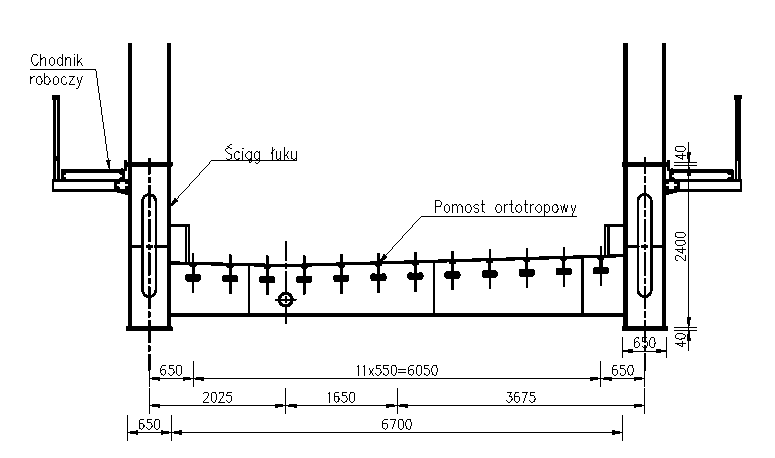
\includegraphics[height=0.25\textheight]{/WK2/rysunki/przekroj_poprzeczny_croped.pdf}} 
 	\captionsetup{justification=centering}
 	\caption{Przekrój poprzeczny przez pomost w strefie podporowej wiaduktu WK2}
 	\label{fig: wk2_cross_sect_deck}
 \end{figure}
 
 W zrealizowanym wariancie pomost został podwieszony do łuku za pomocą prętowych, prostych wieszaków o średnicy 100 mm. Po każdej ze stron zamontowano 12 wieszaków w rozstawie co 5 m. Wieszaki zostały połączone z dźwigarem i ściągiem sztywnym połączeniem spawanym. Rzeczywisty widok zrealizowanego przęsła pokazano na rysunku \ref{fig: wk2_foto_widok_front}, detale konstrukcyjne w obrębie strefy podporowej na rysunku \ref{fig:  wk2_foto_wezglowie}, a połączenie wieszaka ze ściągiem na rysunku \ref{fig: wk2_foto_wieszak}.

\begin{figure}[h]
	\centering
	\subfloat{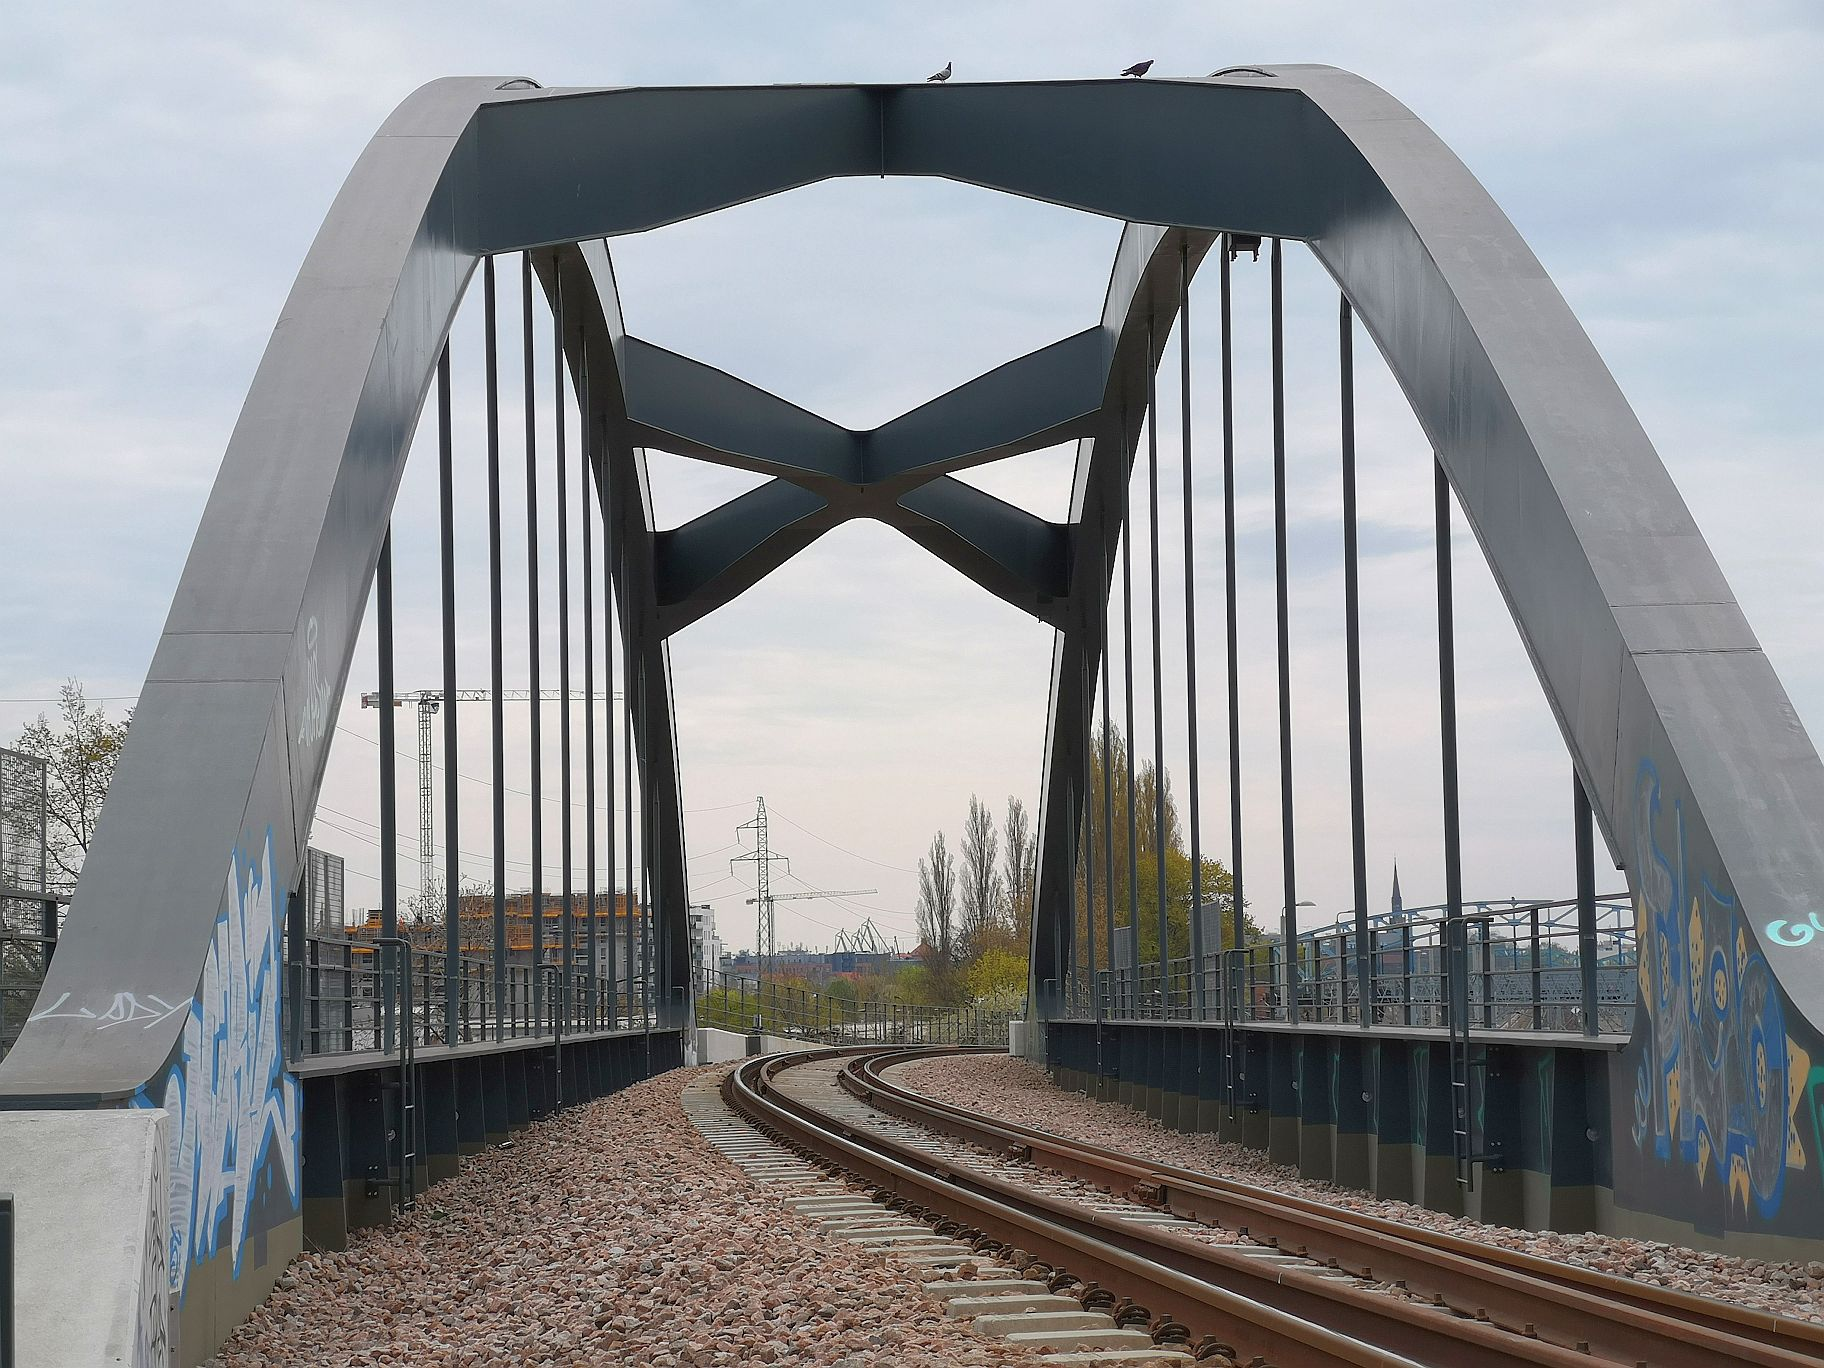
\includegraphics[height=0.30\textheight]{/WK2/zdjecia/widok_front2.jpg}} 
	\captionsetup{justification=centering}
	\caption{Widok od strony lotniska na wiadukt WK2}
	\label{fig: wk2_foto_widok_front}
\end{figure}
\begin{figure}[h]
	\centering
	\subfloat[Widok z góry]{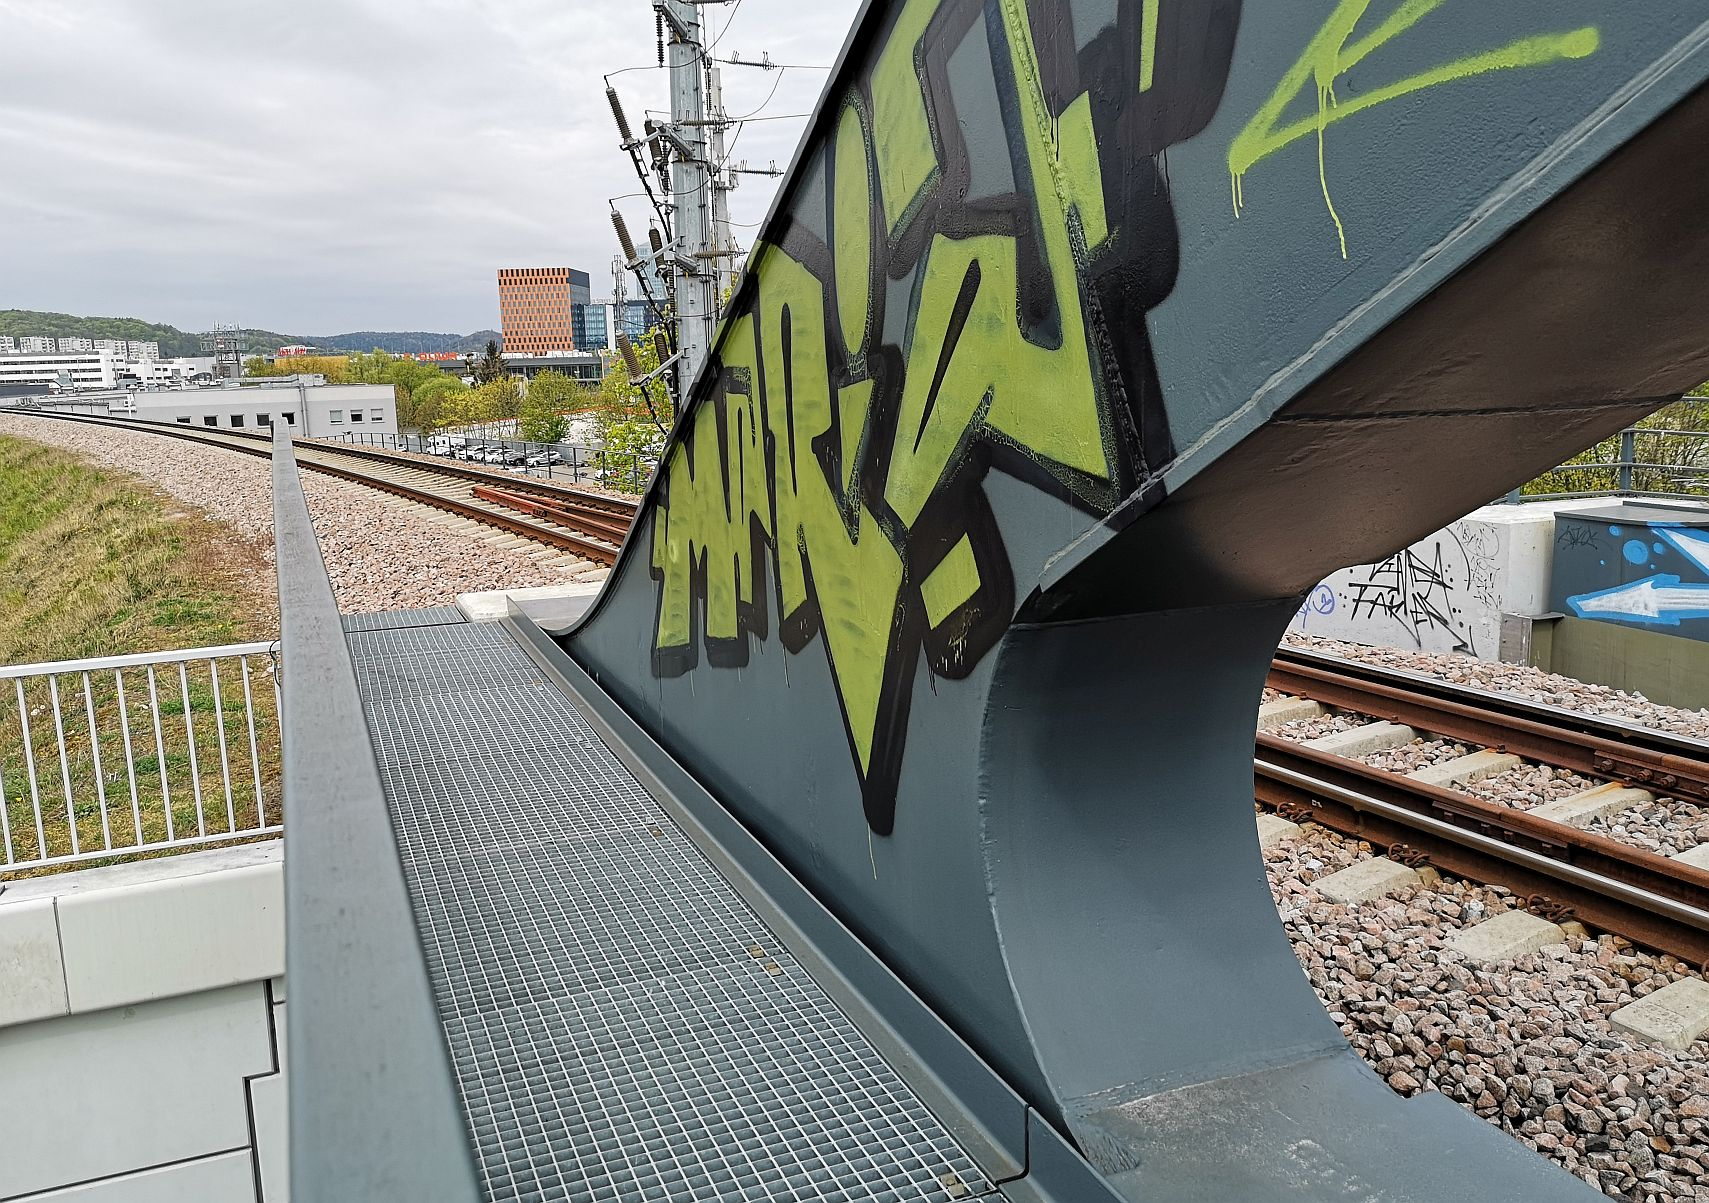
\includegraphics[height=0.2\textheight]{/WK2/zdjecia/wezglowie.jpg}} 
	\qquad
	\subfloat[Widok z dołu]{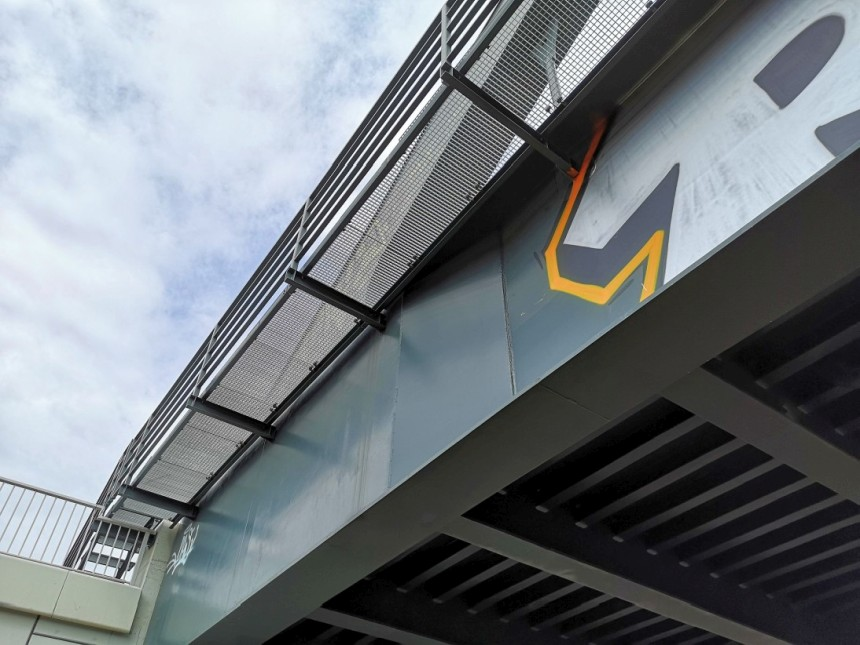
\includegraphics[height=0.2\textheight]{/WK2/zdjecia/detal_wezglowie_dol.jpg}}
	\captionsetup{justification=centering}
	\caption{Szczegóły konstrukcyjne w obrębie połączenia łuku ze ściągiem}
	\label{fig: wk2_foto_wezglowie}
\end{figure}
\begin{figure}[h]
	\centering
	\subfloat{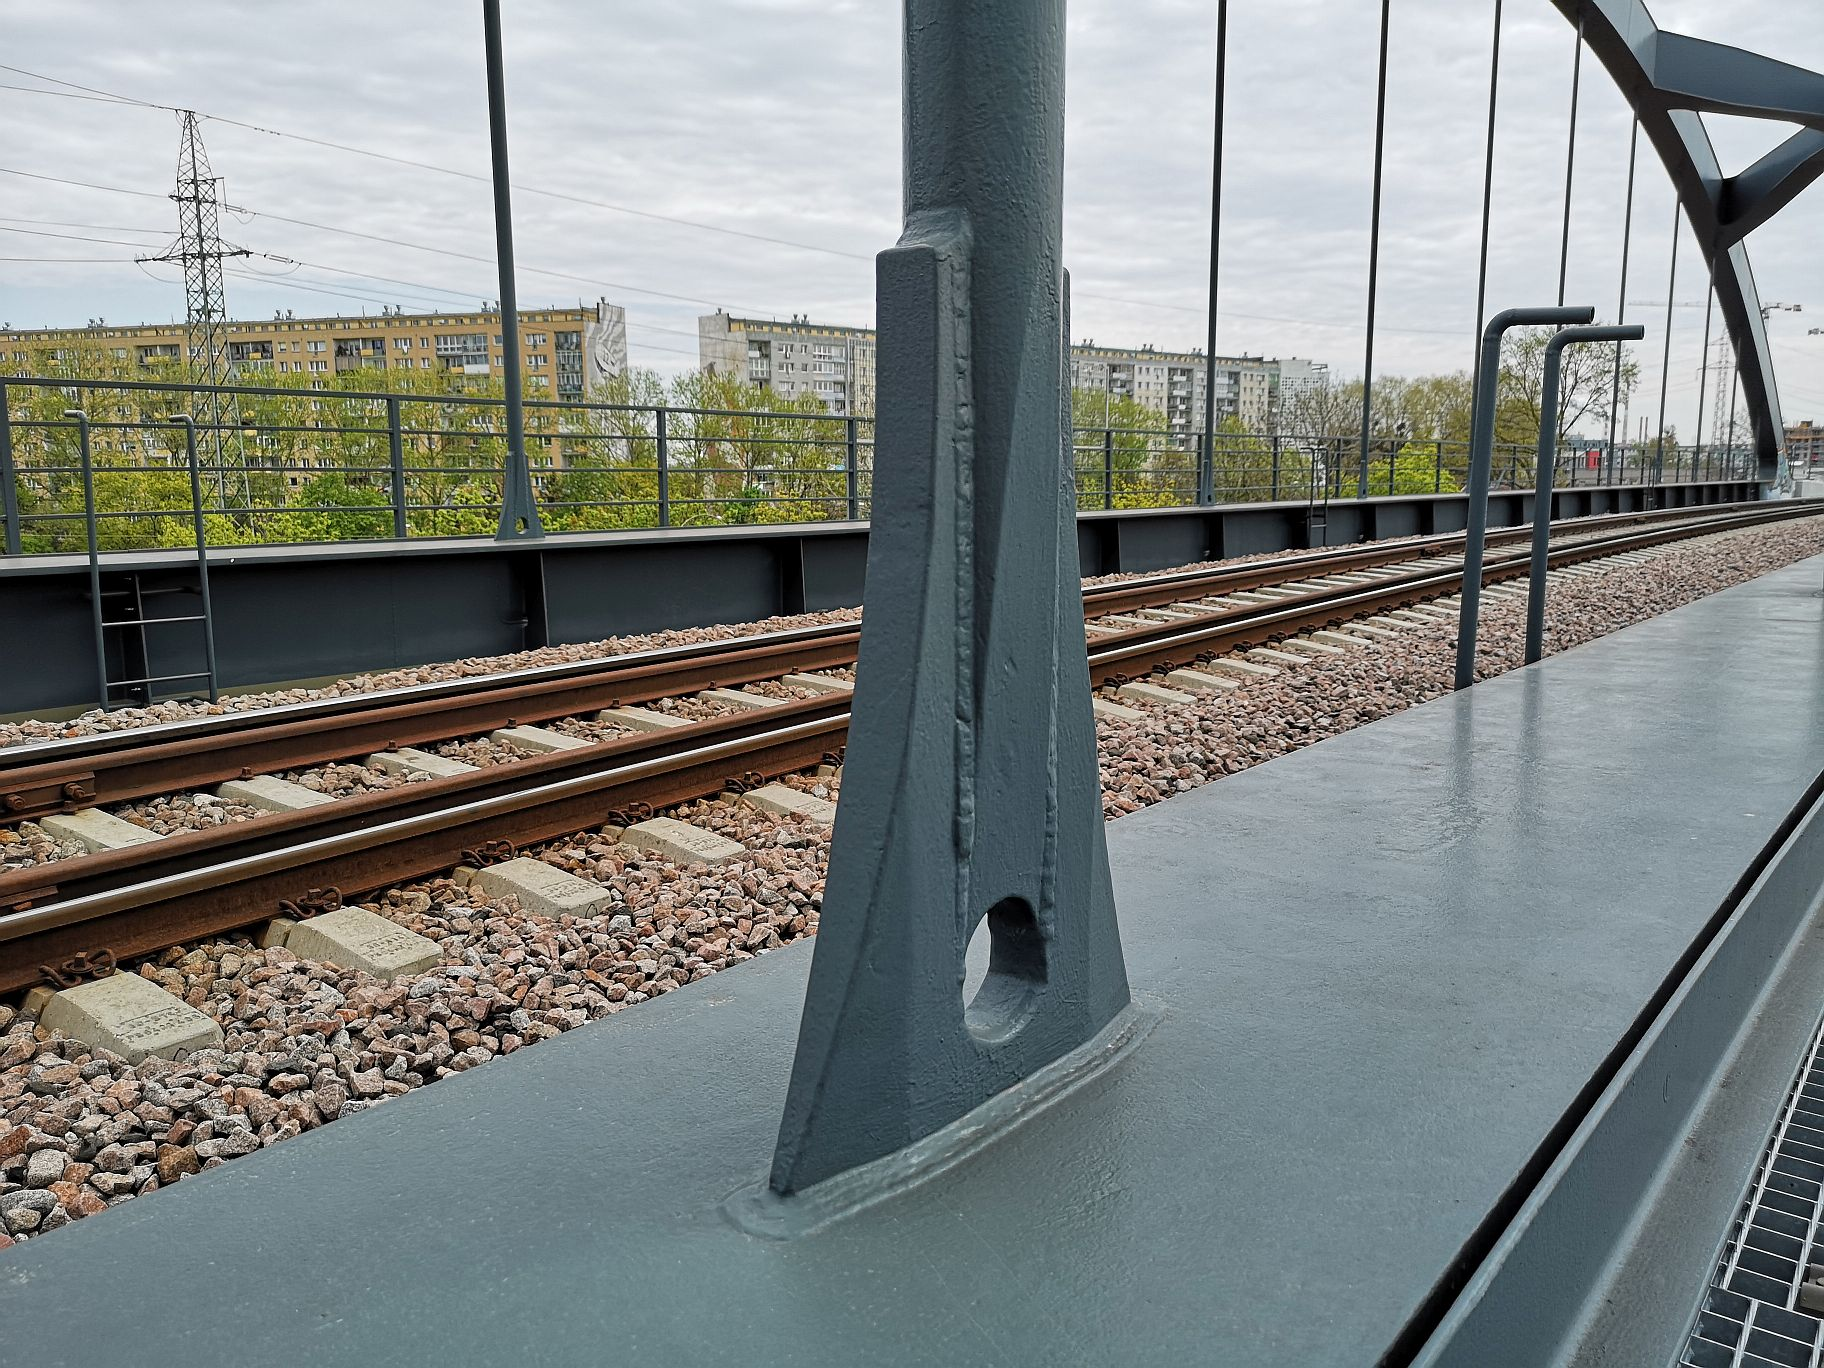
\includegraphics[height=0.2\textheight]{/WK2/zdjecia/zakotwienie_wieszak.jpg}}
	\captionsetup{justification=centering}
	\caption{Detal połączenia wieszaka łuku z pomostem}
	\label{fig: wk2_foto_wieszak}
\end{figure}
Na obiekcie po wybudowaniu przeprowadzono badania odbiorcze. Próbne obciążenia odbyły się w dniu 14.04.2015 i zostały przeprowadzone przez zespół naukowców z Politechniki Śląskiej i Politechniki Gdańskiej \parencite{azinski2015}. Wykonano badania statyczne i dynamiczne. Wyniki jednych i drugich pomiarów posłużą jako elementy kalibracji modelu lub spełnią rolę punktu odniesienia dla wyników badań zrealizowanych w ramach tej pracy. W ramach pomiarów statycznych zrealizowano dwa interesujące, z punktu widzenia tej pracy, ustawienia obciążenia. Ustawienie U1 z obciążeniem zorientowanym symetrycznie na obiekcie oraz ustawienie U2 z obciążeniem wywołującym maksymalne ugięcia w $1/4$ rozpiętości przęsła. Pomiary przemieszczeń wykonywano w 6 punktach zlokalizowanych w $1/4$, $1/2$ i $3/4$ rozpiętości przęsła, po obu jego stronach. Czujniki zamocowano do konstrukcji w osiach ściągów, na dolnych lub górnych pasach. Obciążenie statyczne stanowiły dwie lokomotywy spalinowe typu: SM-48 i BR232. Pomierzone ugięcia statyczne zostaną użyte jako dodatkowe kyterium kalibracji modelu numerycznego.
W ramach badań dynamicznych mierzono przyspieszenia konstrukcji po wymuszeniu obciążeniem impulsowym. Impuls generowano przez upadek jednej osi koparki dwudrogowej i zeskoków drezyny z progu. Na postawie przebiegów drgań swobodnych zidentyfikowano częstotliwości drgań własnych przęsła i towarzyszące im tłumienia. Do identyfikacji użyto algorytmu ERA. Zidentyfikowane częstotliwości drgań i tłumienia przęsła posłużą do porównania z wynikami badań przeprowadzonymi w ramach tej pracy.


\section{Budowa modelu numerycznego}

Na potrzeby analiz numerycznych zbudowano model MES w środowisku SOFiSTiK (rys. \ref{fig: model_wk2_visualization}) Model przestrzenny składa się kilku rodzajów elementów skończonych. Z jednowymiarowych elementów belkowych wykonano łuki, stężenia, belki ściągu, wzmocnienia wezgłowii i żebra pomostu ortotropowego. Z elementów kratowych stworzono wieszaki. Blachę pomostu wykonano z czterowęzłowych elementów powłokowych. Połączenia pomiędzy końcami wieszaków i osiami łuku oraz ściągu zrealizowano przez połączenia kinematyczne translacji i rotacji węzłów. Podparcia pionowe w miejscach łożysk mostu zrealizowano za pomocą sztywnych więzów węzłów. Nie zablokowano przesuwów podłużnych i poprzecznych za pomocą blokady przemieszczeń. Zamiast tego na obu kierunkach zamocowano elastyczne elementy o bardzo dużej sztywności. Dostosowanie do istniejących warunków łożyskowania opisane zostało w dalszej części rozdziału. Usztywnienia wezgłowii zamodelowano za pomocą rusztu elementów belkowych o przekroju składającym się z dwóch blach odsuniętych od siebie na szerokość przekroju skrzynkowego łuku. Elementy strukturalne konstrukcji (takie jak ściągi, pomost, dźwigary łukowe, elementy podparcia itd.) podzielono w modelu na grupy pozwalające odnosić się do nich jako całości. Przekroje elementów belkowych przyjęto zgodnie z dostępną dokumentacją (!!!). Wymiary przekrojów zmiennych po długości zostały interpolowane liniowo. Widoczne na rysunku (\ref{fig: model_wk2_static_scheme}) dodatkowe połączenia kinematyczne są przygotowaniem dla możliwości podłączenia innych konfiguracji wieszaków.



\begin{figure}[h]
	\centering
	\subfloat[Widok A]{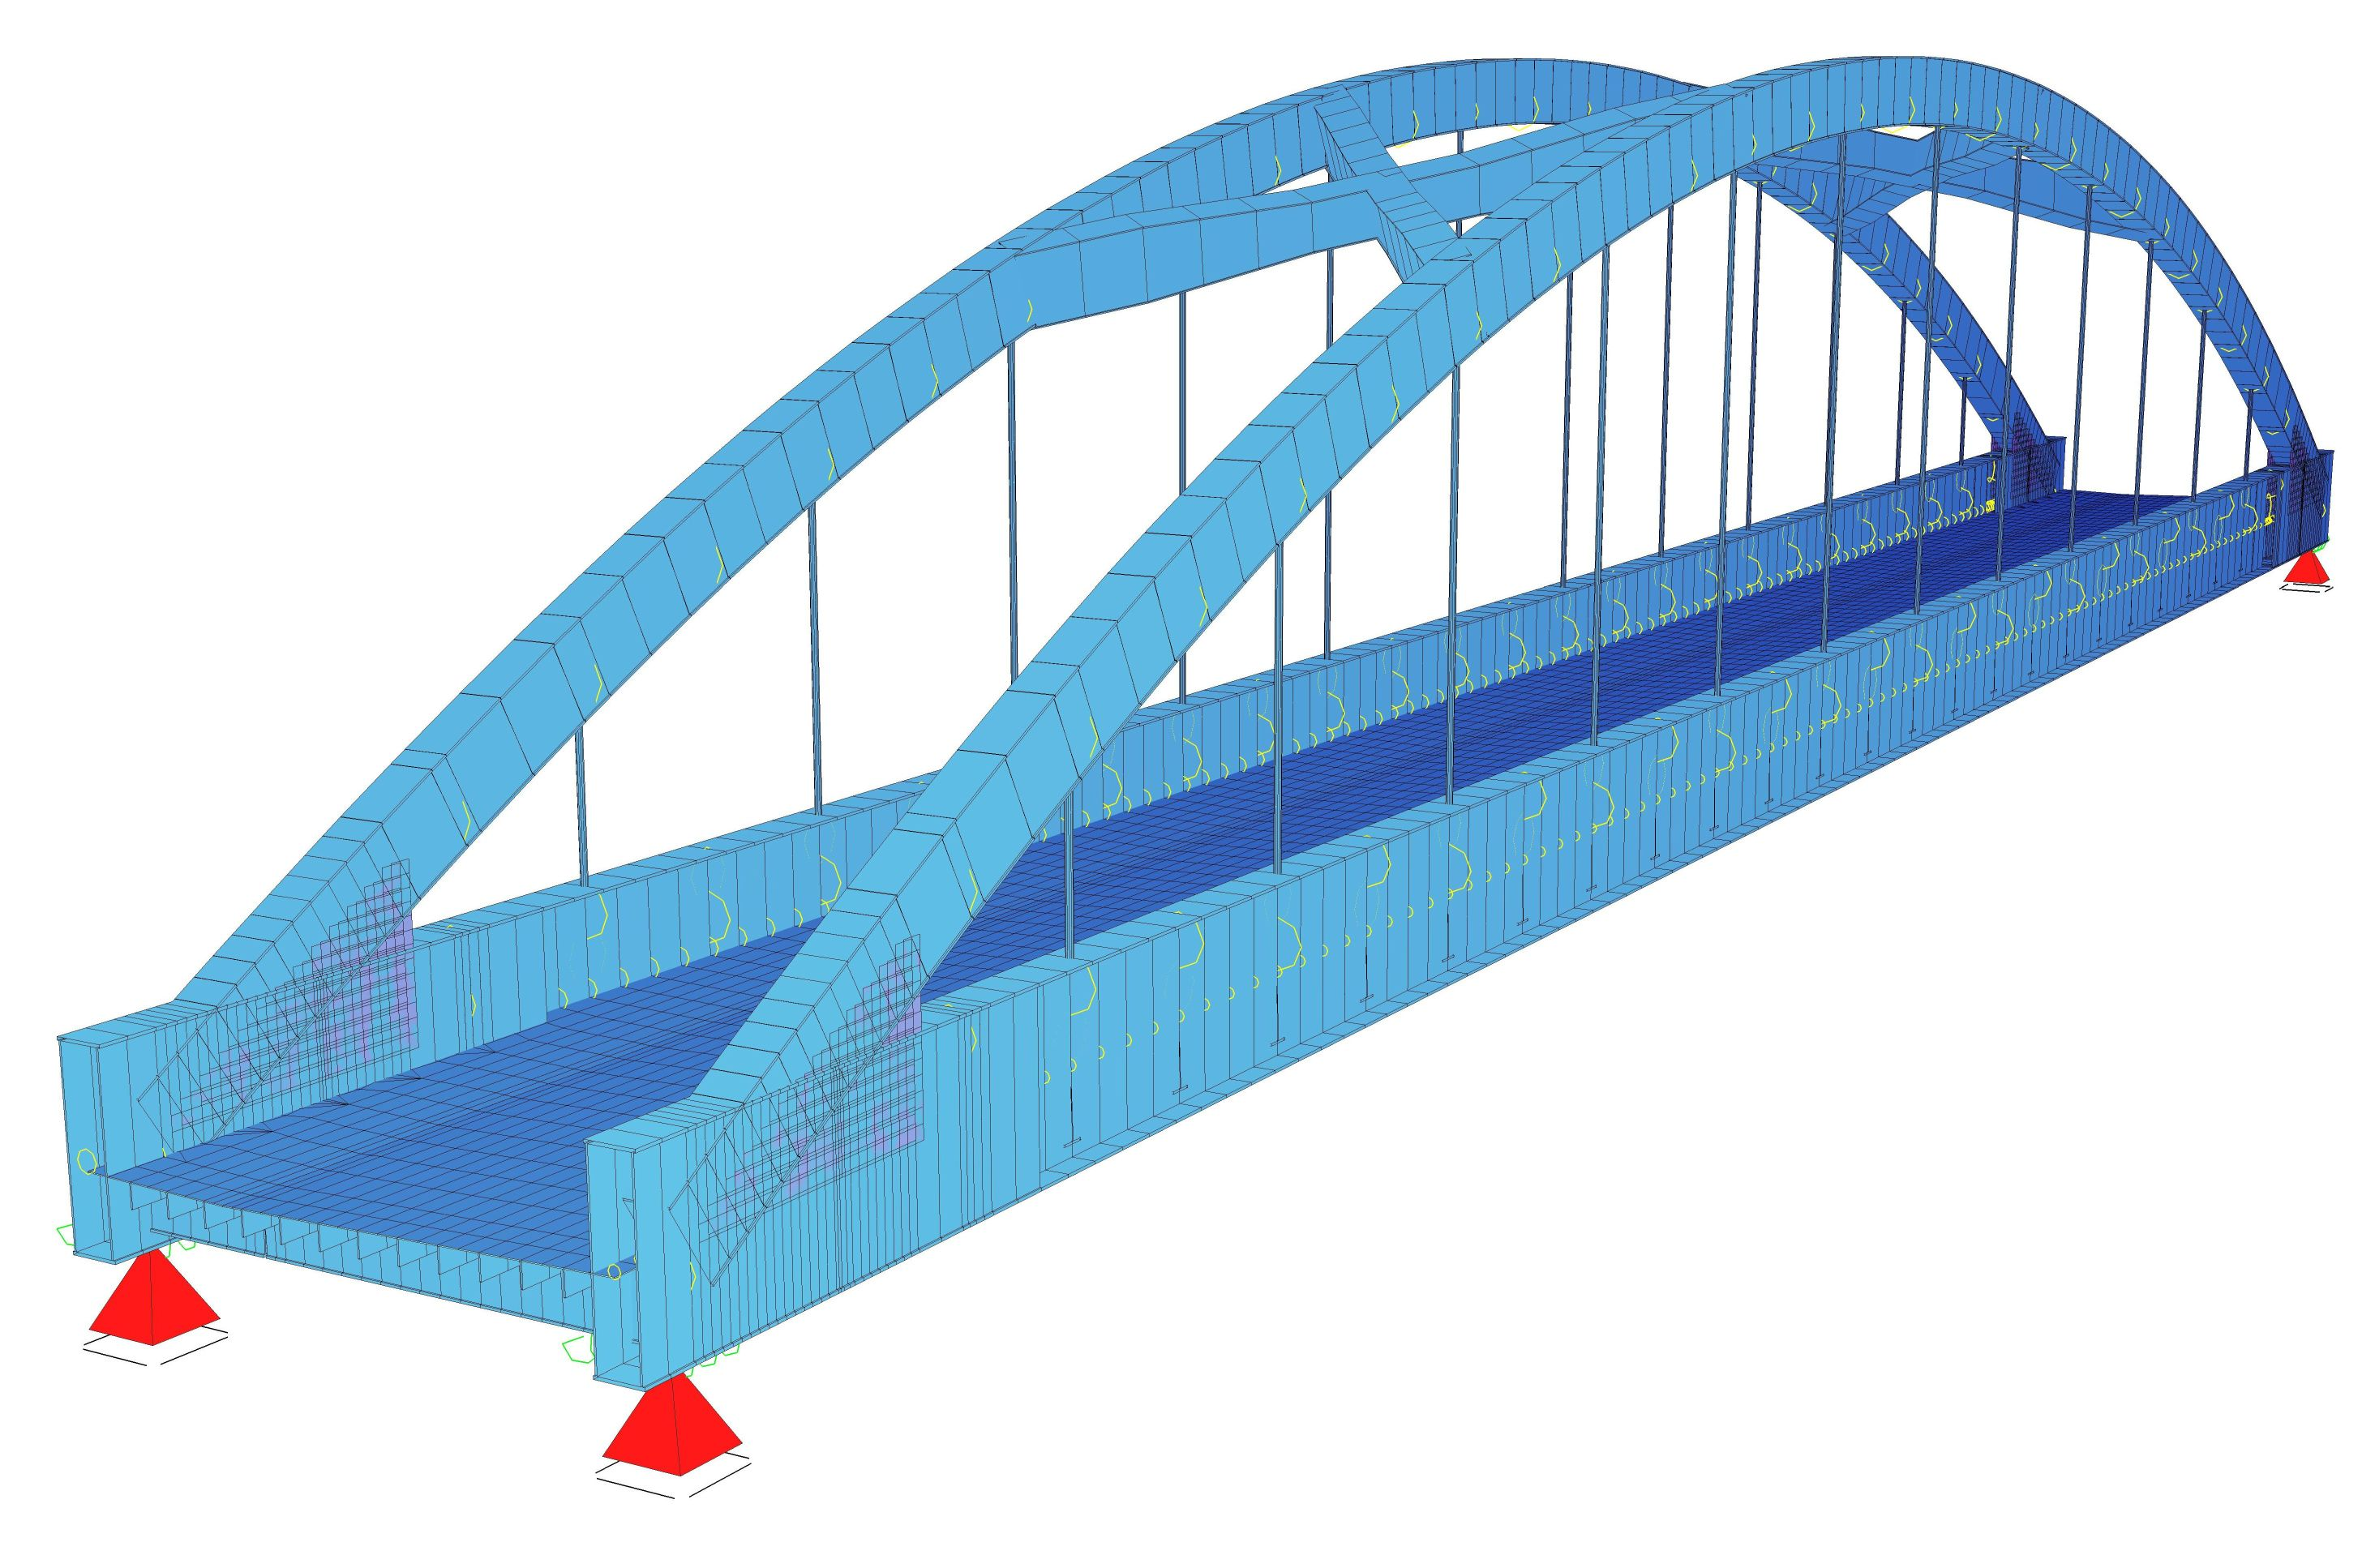
\includegraphics[width=0.5\linewidth]{/WK2/model/SCIAG_PAR_v01_vis_1.jpg}}%
	\subfloat[Widok B]{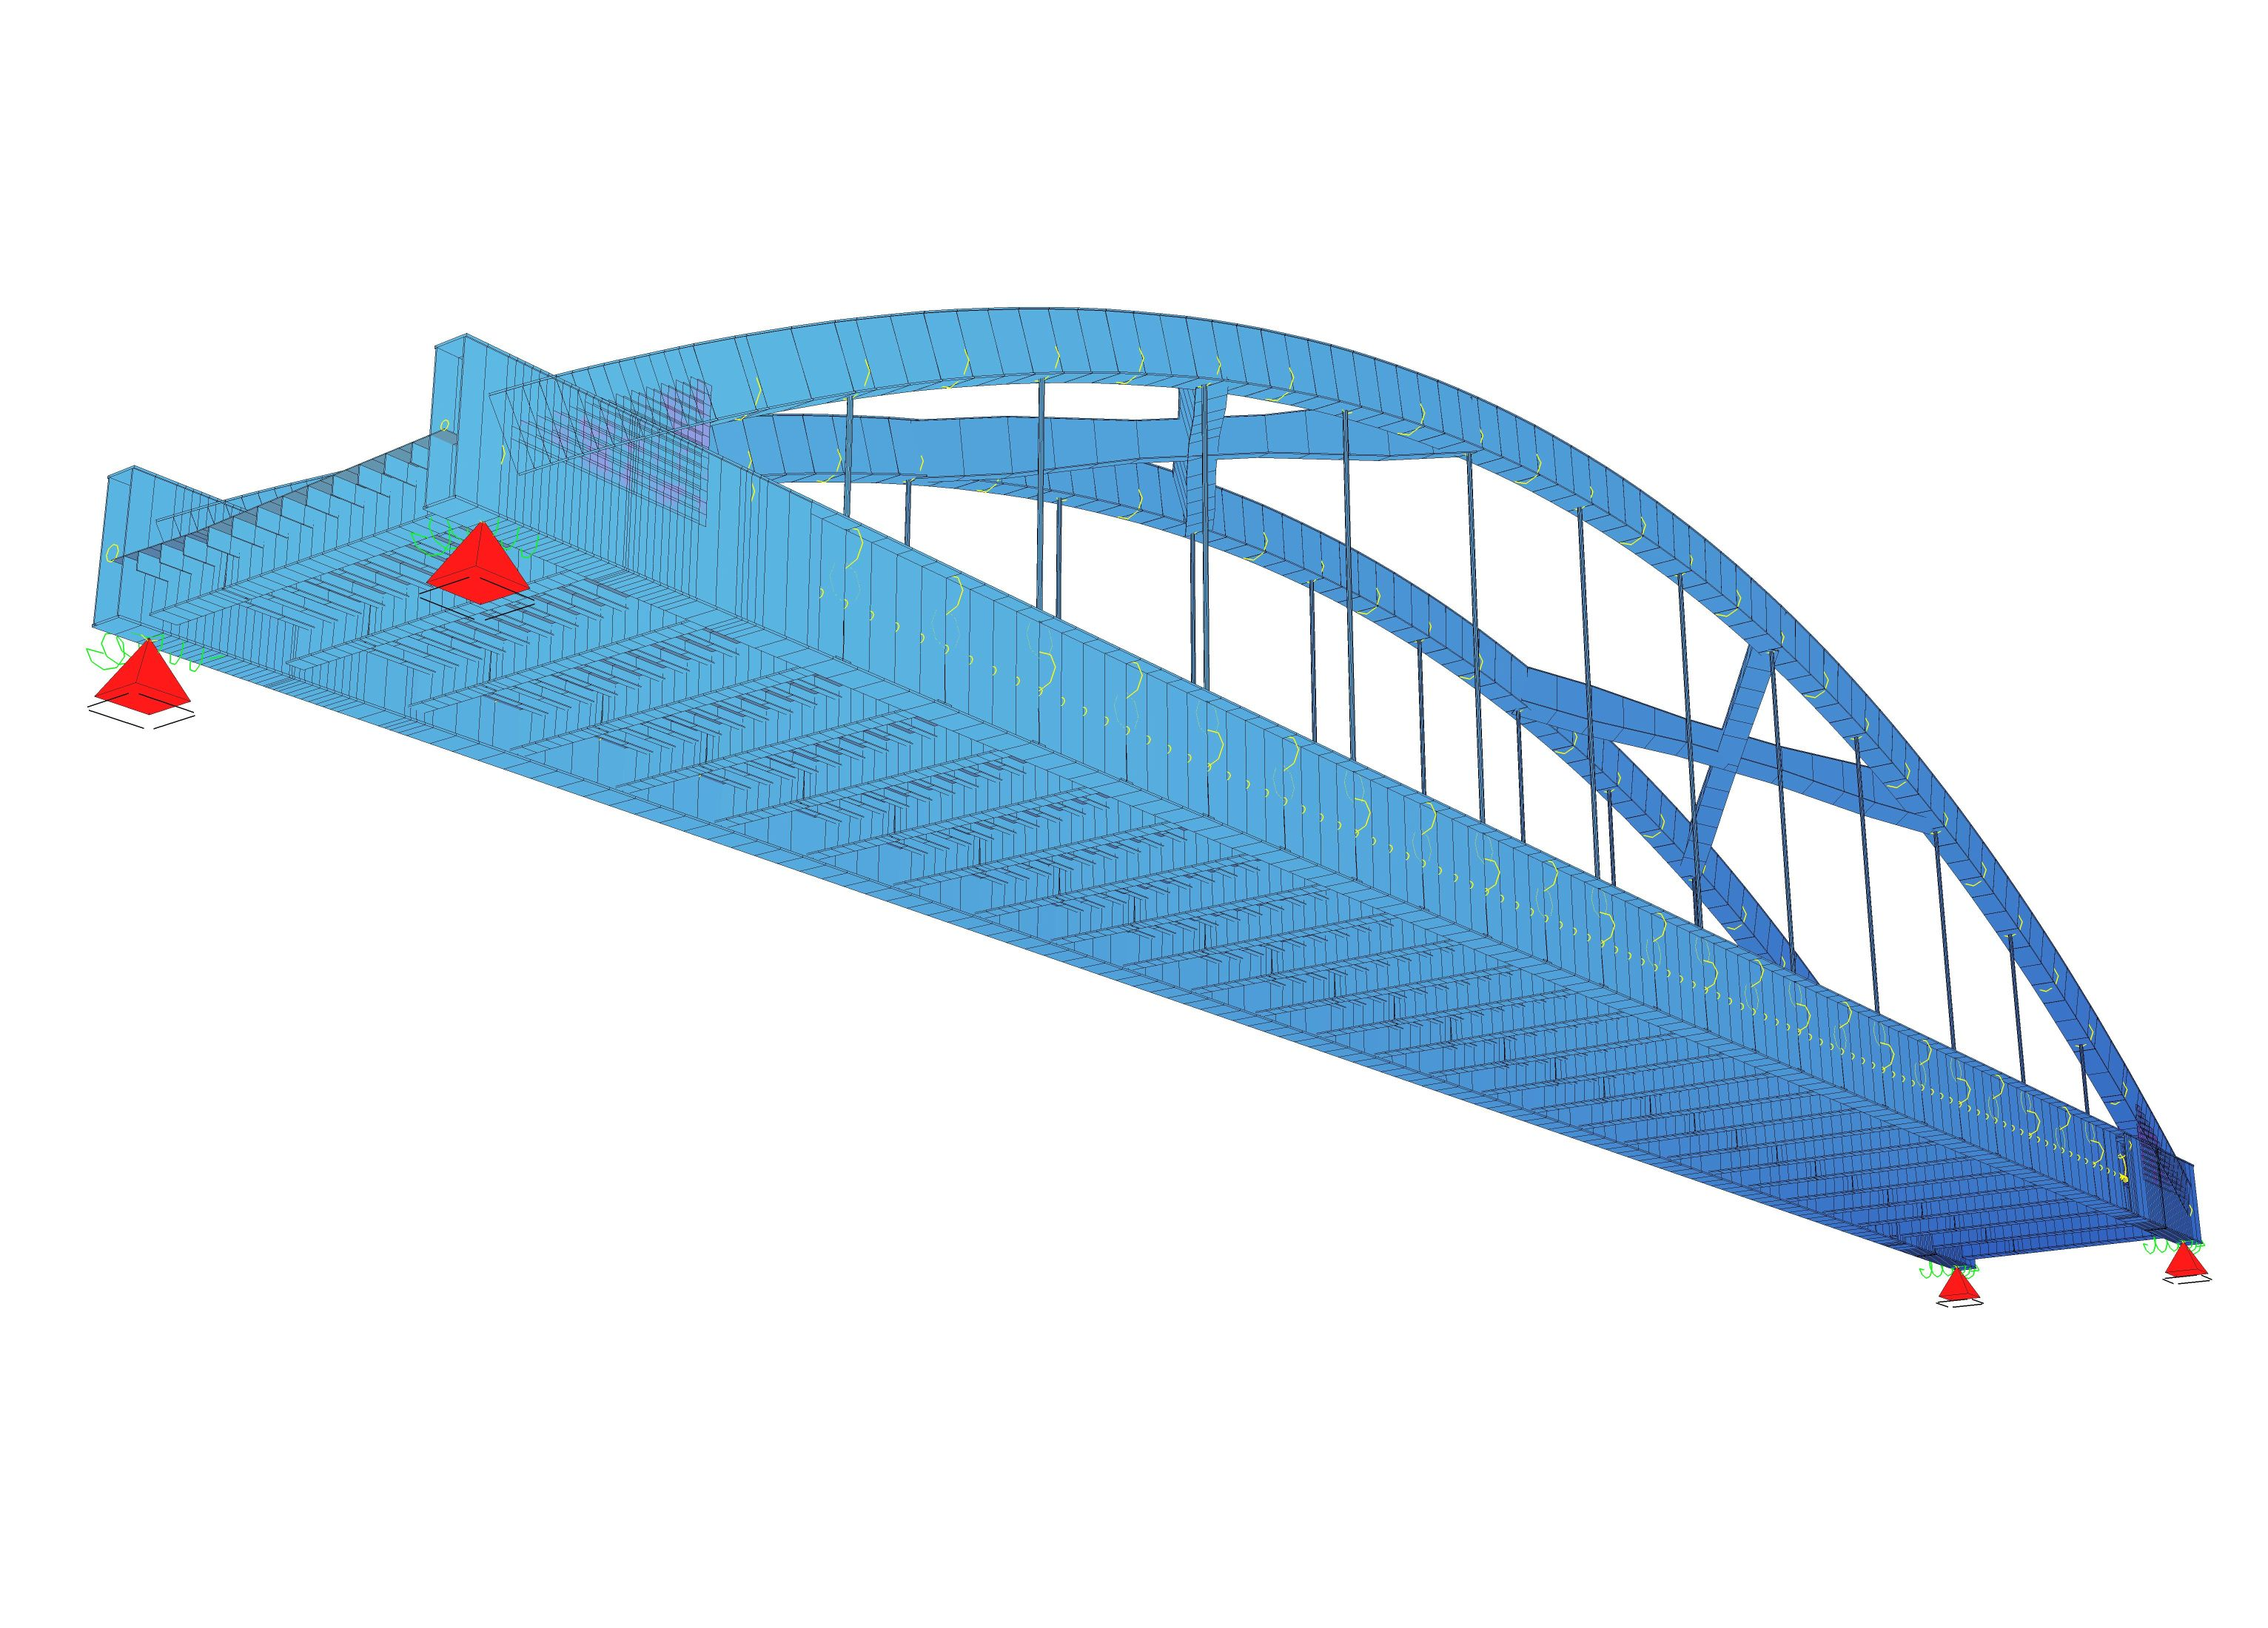
\includegraphics[width=0.5\linewidth]{/WK2/model/SCIAG_PAR_v01_vis_2.jpg}}
	\captionsetup{justification=centering}
	\caption{PODMIENIC NA RZECZYWISTE WYMIARY KONSTRUKCJI!!!!! Wizualizacja przestrzennego modelu numerycznego wiaduktu WK2 Pomorskiej Kolei Metropolitalnej}
	\label{fig: model_wk2_visualization}
	
\end{figure}
\begin{figure}[h]
	\centering
	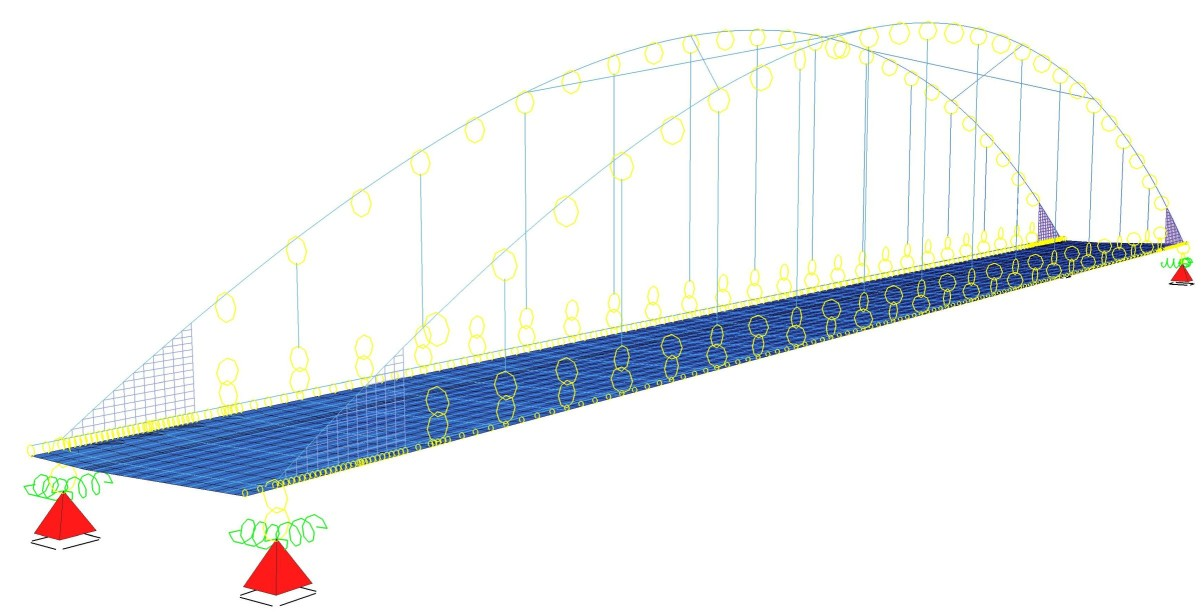
\includegraphics[width=0.5\linewidth]{/WK2/model/SCIAG_PAR_v01_schemat_1.jpg}
	\captionsetup{justification=centering}
	\caption{Schemat statyczny modelu numerycznego wiaduktu WK2 Pomorskiej Kolei Metropolitalnej}
	\label{fig: model_wk2_static_scheme}
\end{figure}

Obciążenie ciężarem własnym konstrukcji zostało wygenerowane na podstawie ciężarów wprowadzonych przekrojów elementów liniowych bądź grubości elementów powłokowych. Dodatkowe elementy takie jak przepony i zakotwienia wieszaków dodane zostały jako obciążenia węzłowe. Osobny przypadek obciążenia stanowi pomost roboczy dodany jako ekwiwalentne obciążenie węzłowe i momenty zginające. Ostatnim obciążeniem stałym jest ciężar tłucznia. Z uwagi na ułożenie toru po łuku w planie, rozkład tłucznia na obiekcie nie jest regularną, symetryczną bryłą. Dostępna dokumentacja obiektu nie dostarcza dokładnych informacji o ułożeniu podsypki na pomoście. Podsypka została w prosty sposób zinwentaryzowana przez pomiar grubości w niektórych punktach charakterystycznych. Na rysunku \ref{fig: wk2_cross_sect} zaprezentowano zinwentaryzowany układ tłucznia w przekroju przęsłowym. Zastosowana metoda pomiaru objętości tłucznia nie jest dokładna i na pewno nie odzwierciedla realnego rozkładu ciężaru podsypki na obiekcie. Z tego względu podzielono obciążenie tłuczniem na dwa osobne przypadki: równomiernie rozłożone obciążenie na całym pomoście i obciążenie równomierne o szerokości (!!!) usytuowane wzdłuż osi toru. Wartość obciążenia tłuczniem przyjęto z normy (!!!).
\begin{figure}[p]
	\centering
	\begin{tabular}[c]{c}
		\subfloat[Mod 1, $f_1=1.408\text{ Hz}$]{\label{fig: wk2_origin_mod01}%
			\begin{tabular}[b]{c c}
				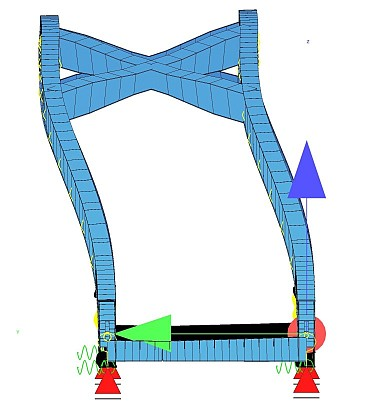
\includegraphics[height=0.12\textheight]{/WK2/model/mod_origin/f1f.jpg}%
				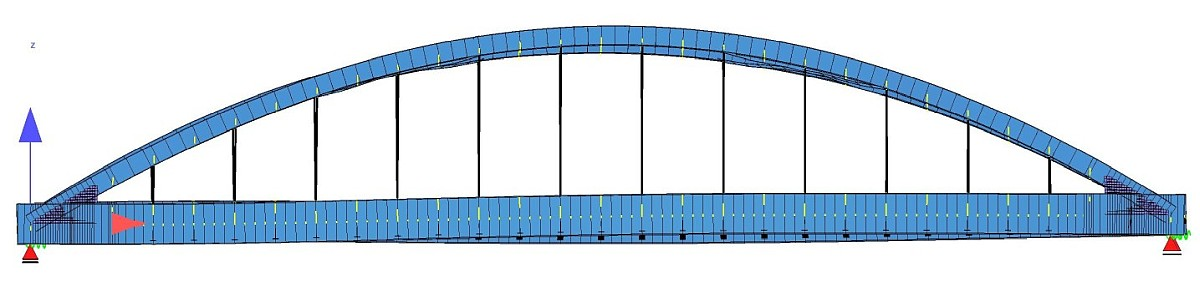
\includegraphics[width=0.7\textwidth]{/WK2/model/mod_origin/f1s.jpg}%
		\end{tabular}}\\
		\subfloat[Mod 2, $f_2=2.469 \text{ Hz}$]{\label{fig: wk2_origin_mod02}%
		\begin{tabular}[b]{c c}
			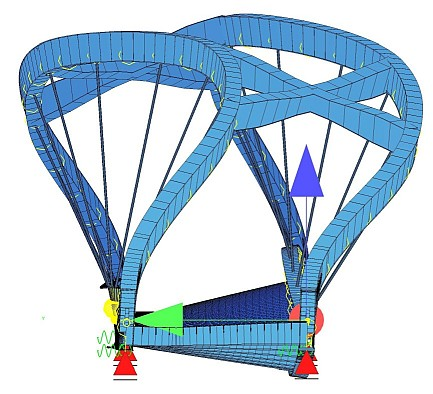
\includegraphics[height=0.12\textheight]{/WK2/model/mod_origin/f2f.jpg}%
			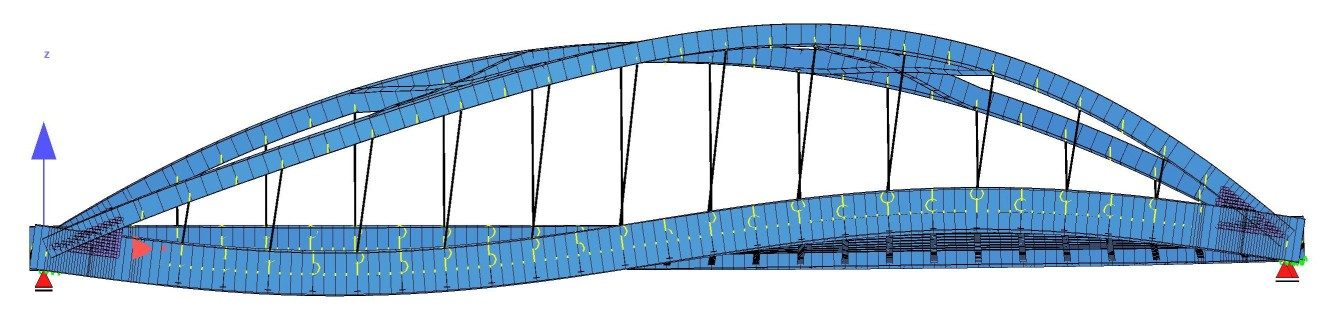
\includegraphics[width=0.7\textwidth]{/WK2/model/mod_origin/f2s.jpg}%
		\end{tabular}}\\
			\subfloat[Mod 3, $f_3=2.509 \text{ Hz}$]{\label{fig: wk2_origin_mod03}%
		\begin{tabular}[b]{c c}
			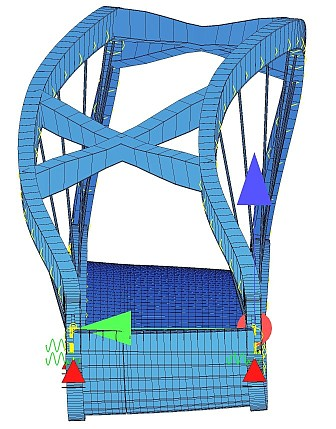
\includegraphics[height=0.12\textheight]{/WK2/model/mod_origin/f3f.jpg}%
			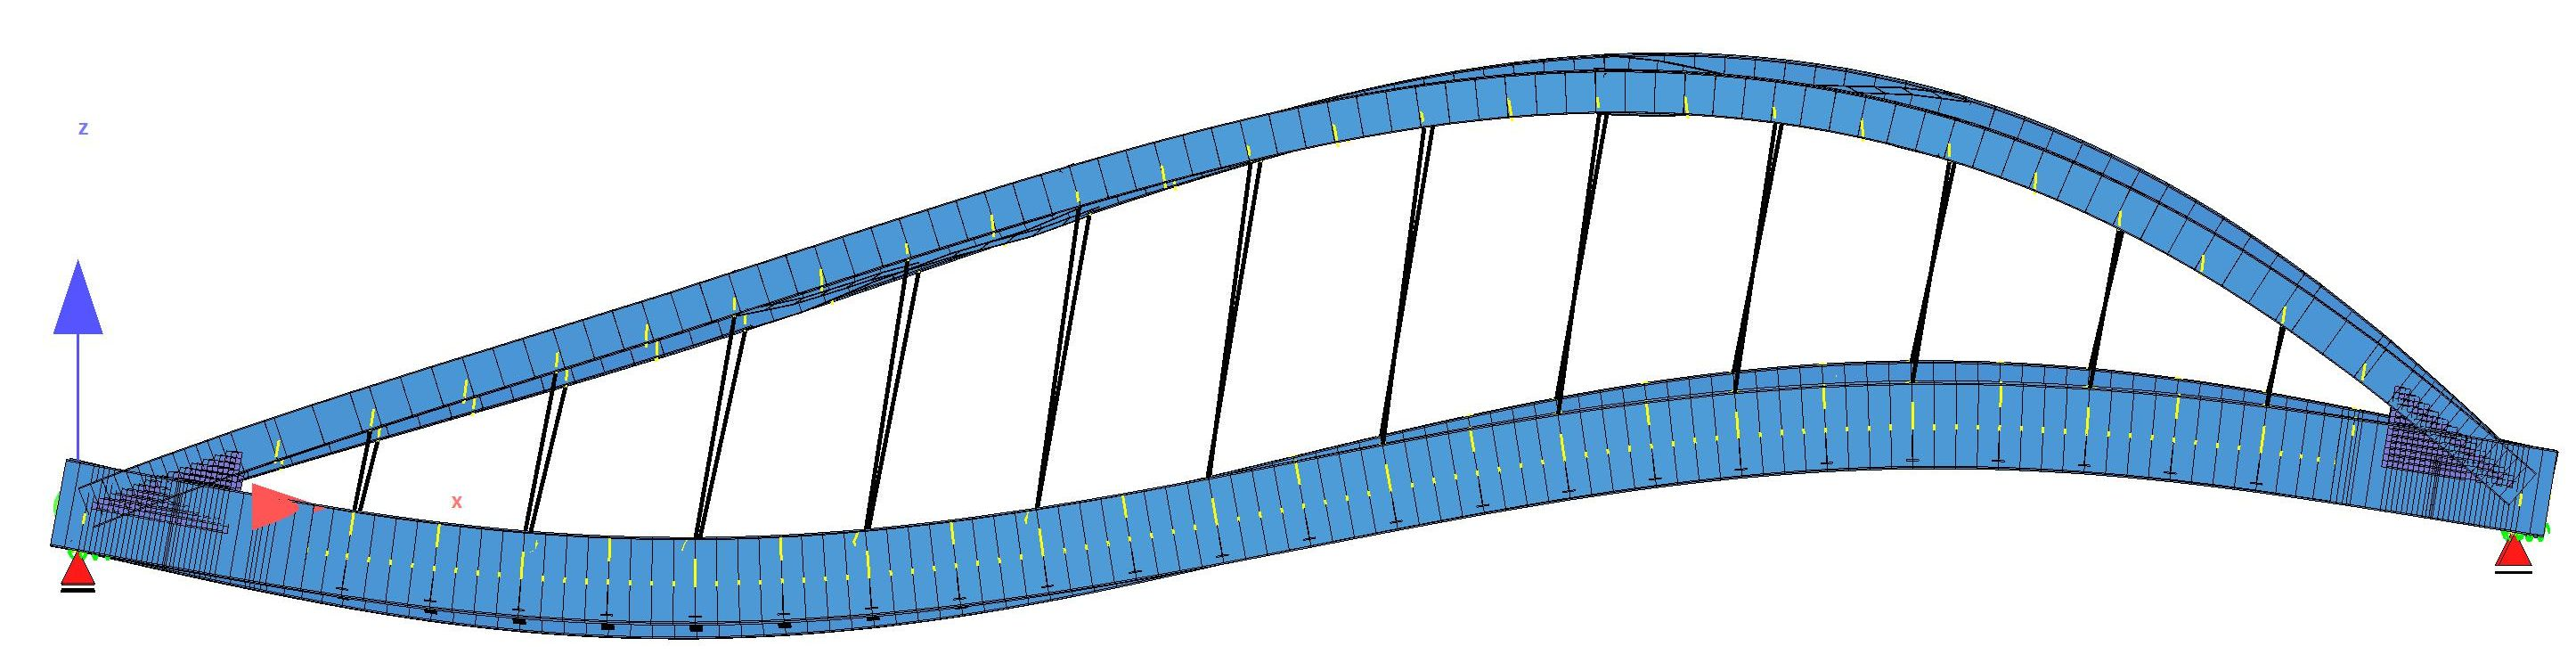
\includegraphics[width=0.7\textwidth]{/WK2/model/mod_origin/f3s.jpg}%
	\end{tabular}}\\
		\subfloat[Mod 4, $f_4=3.166 \text{ Hz}$]{\label{fig: wk2_origin_mod04}%
	\begin{tabular}[b]{c c}
		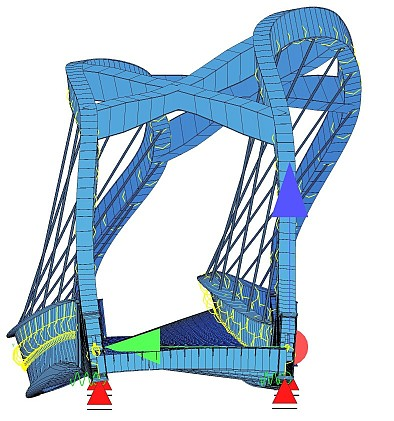
\includegraphics[height=0.12\textheight]{/WK2/model/mod_origin/f4f.jpg}%
		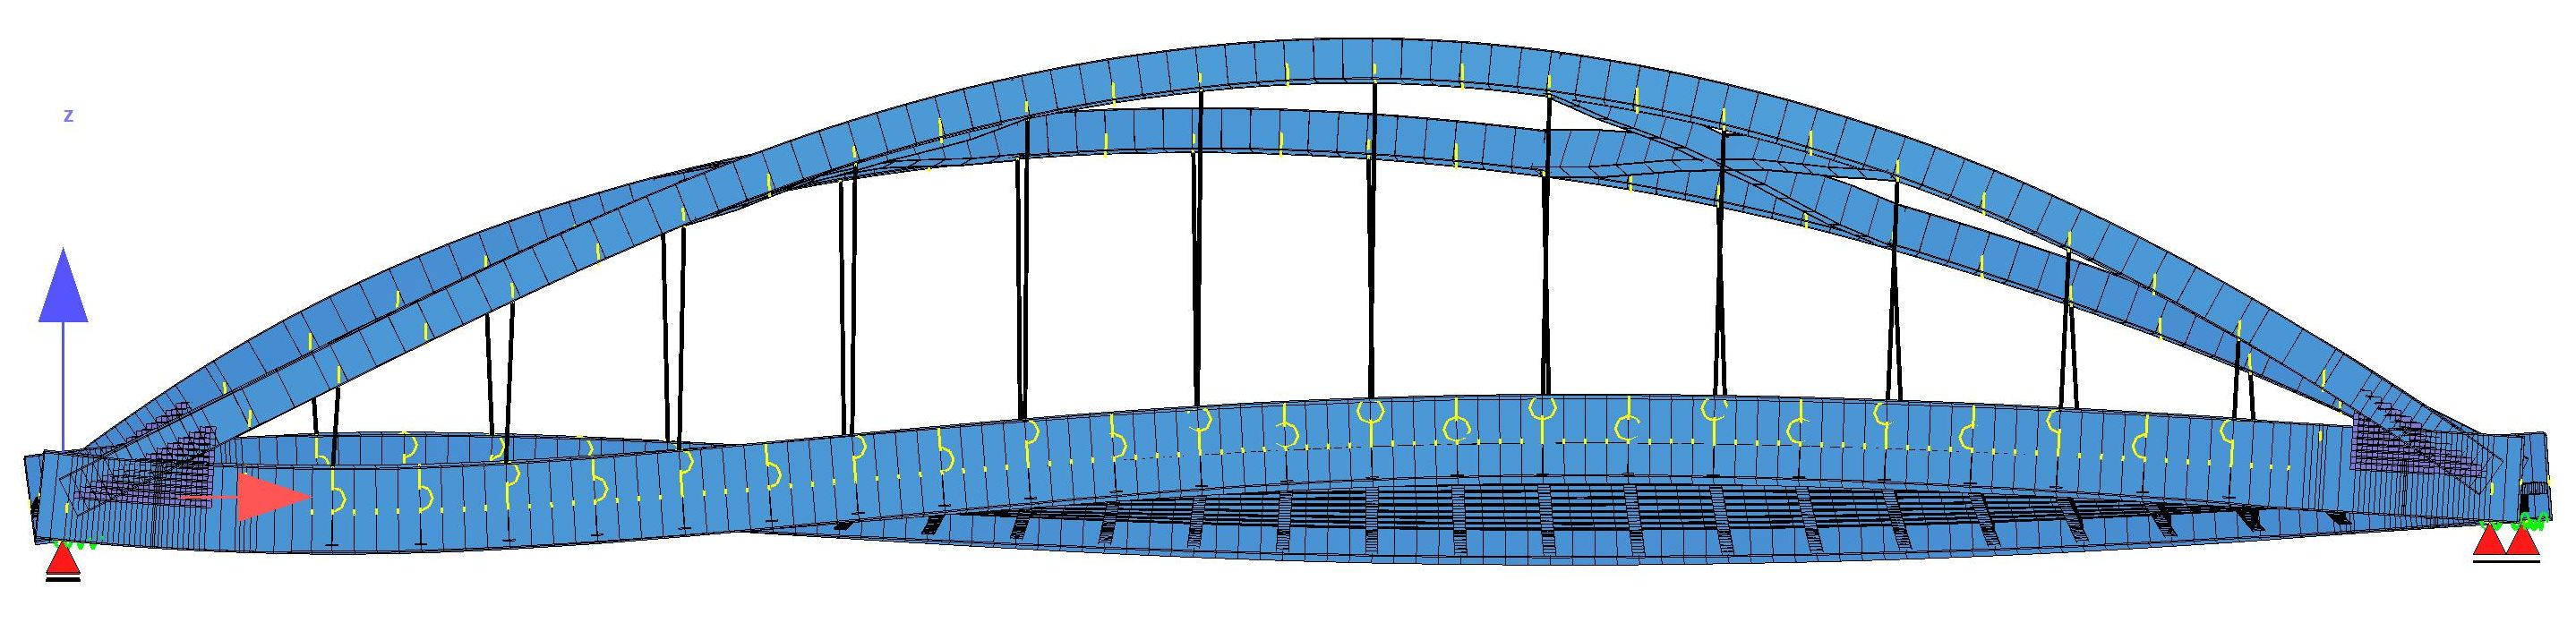
\includegraphics[width=0.7\textwidth]{/WK2/model/mod_origin/f4s.jpg}%
\end{tabular}}\\
		\subfloat[Mod 5, $f_5=3.515 \text{ Hz}$]{\label{fig: wk2_origin_mod05}%
	\begin{tabular}[b]{c c}
		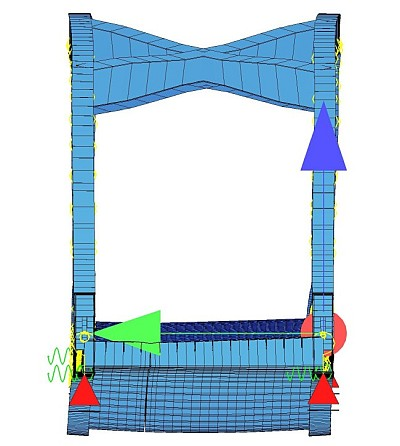
\includegraphics[height=0.12\textheight]{/WK2/model/mod_origin/f5f.jpg}%
		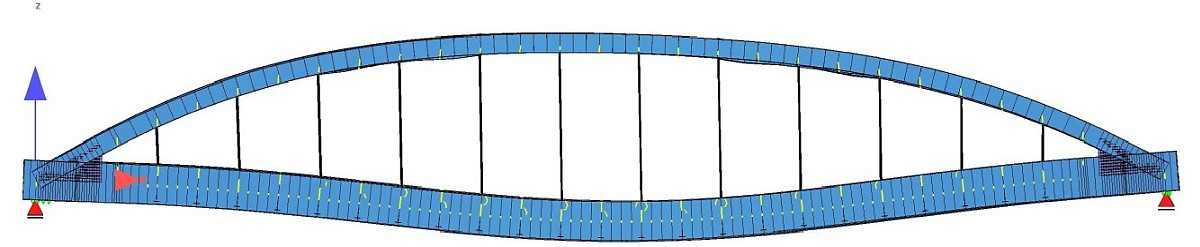
\includegraphics[width=0.7\textwidth]{/WK2/model/mod_origin/f5s.jpg}%
\end{tabular}}\\
		\subfloat[Mod 6, $f_6=5.031 \text{ Hz}$]{\label{fig: wk2_origin_mod06}%
	\begin{tabular}[b]{c c}
		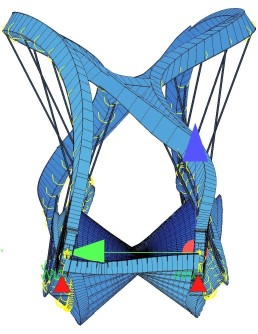
\includegraphics[height=0.12\textheight]{/WK2/model/mod_origin/f6f.jpg}%
		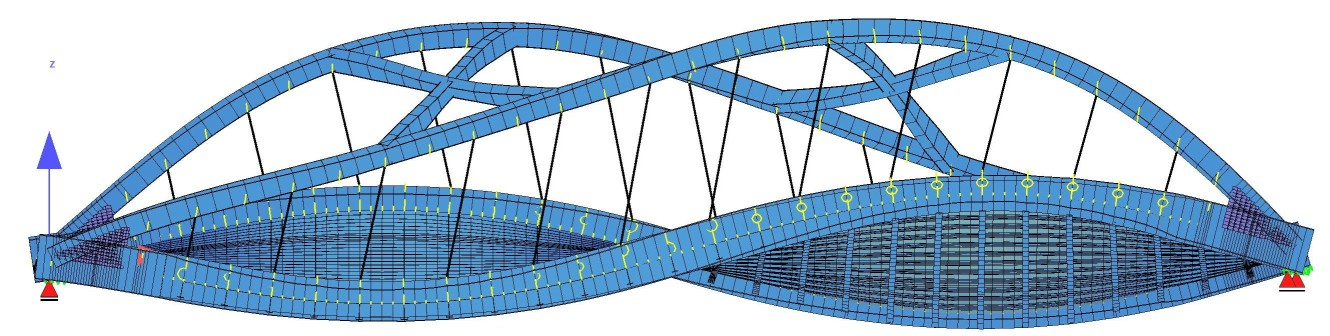
\includegraphics[width=0.7\textwidth]{/WK2/model/mod_origin/f6s.jpg}%
\end{tabular}}\\
	\end{tabular}
	\caption{Postaci i częstotliwości drgań własnych wiaduktu WK2 - Model wstępny}
	\label{fig: model_wk2_origin_mods}
\end{figure}

\begin{figure}[H]\ContinuedFloat
	\centering
	\begin{tabular}[c]{c}
		\subfloat[Mod 7, $f_7=5.584 \text{ Hz}$]{\label{fig: wk2_origin_mod07}%
			\begin{tabular}[b]{c c}
				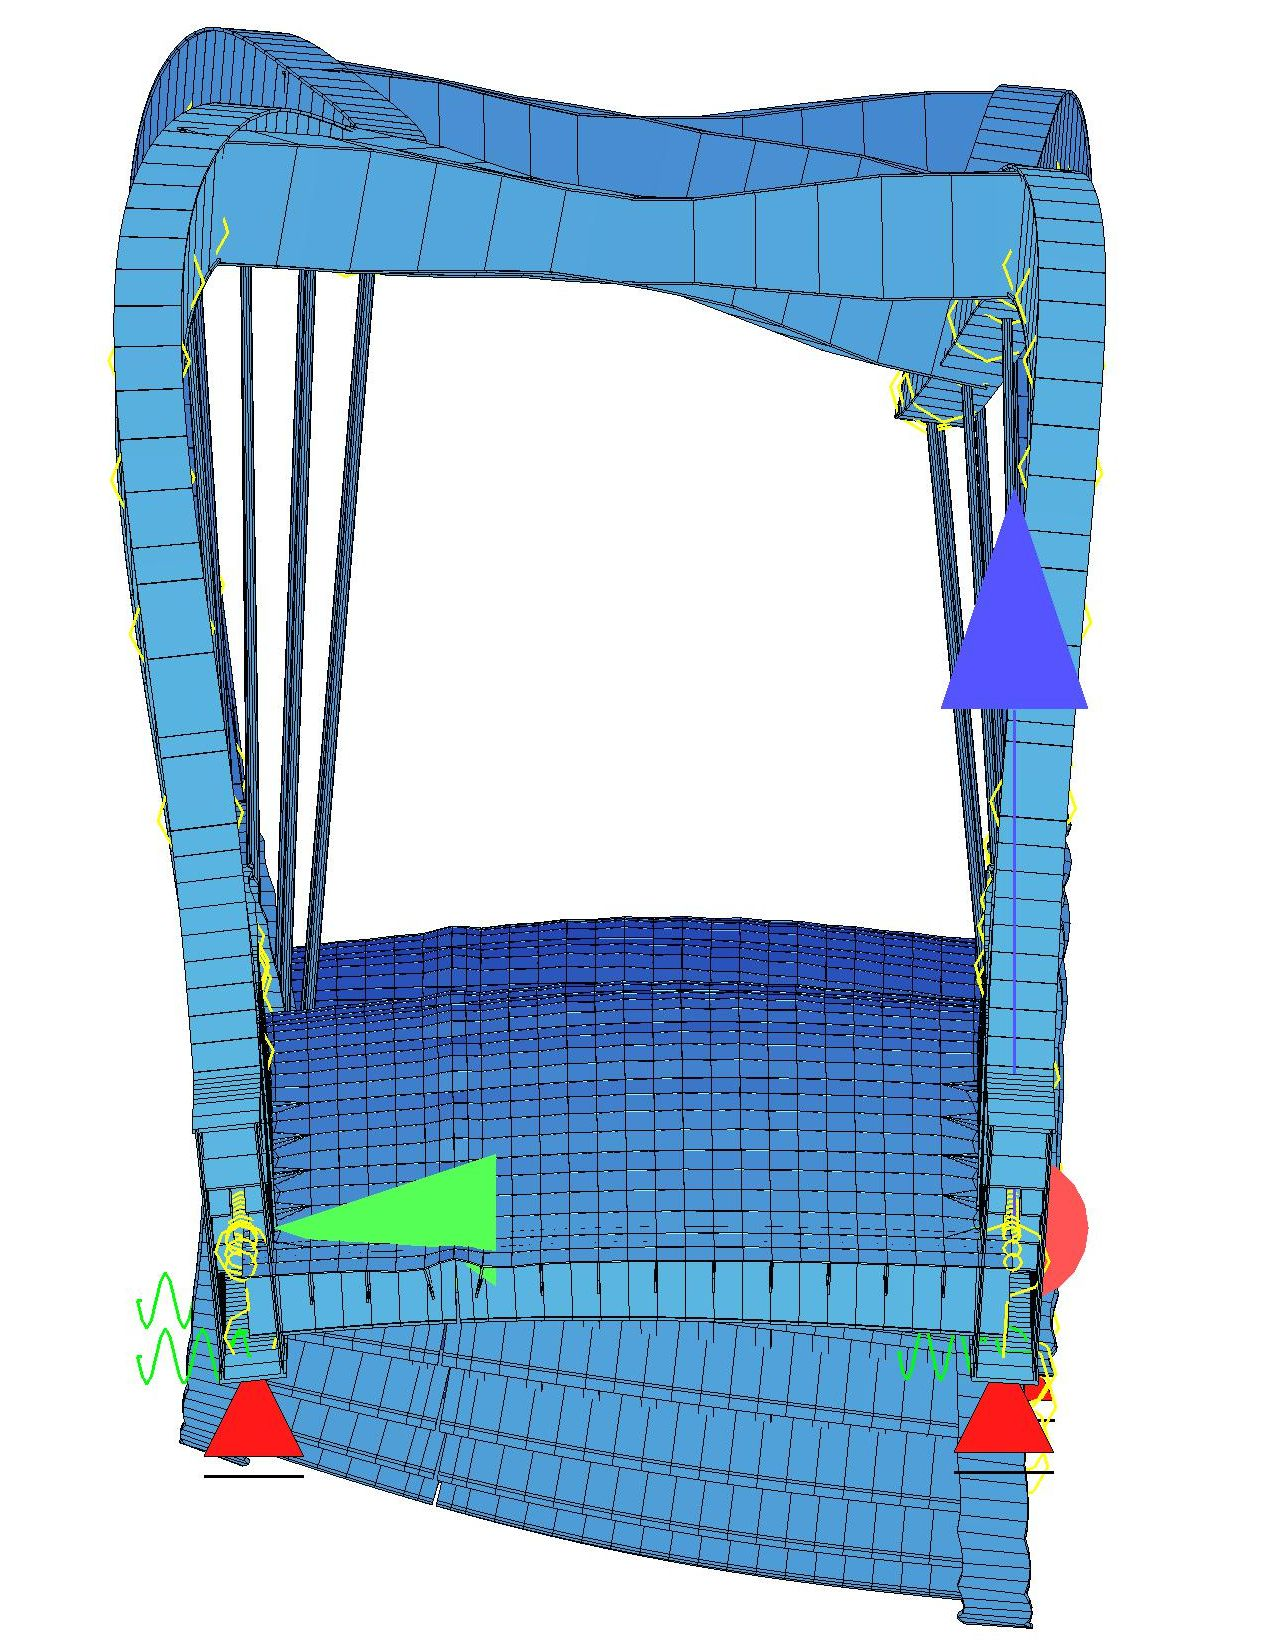
\includegraphics[height=0.12\textheight]{/WK2/model/mod_origin/f7f.jpg}%
				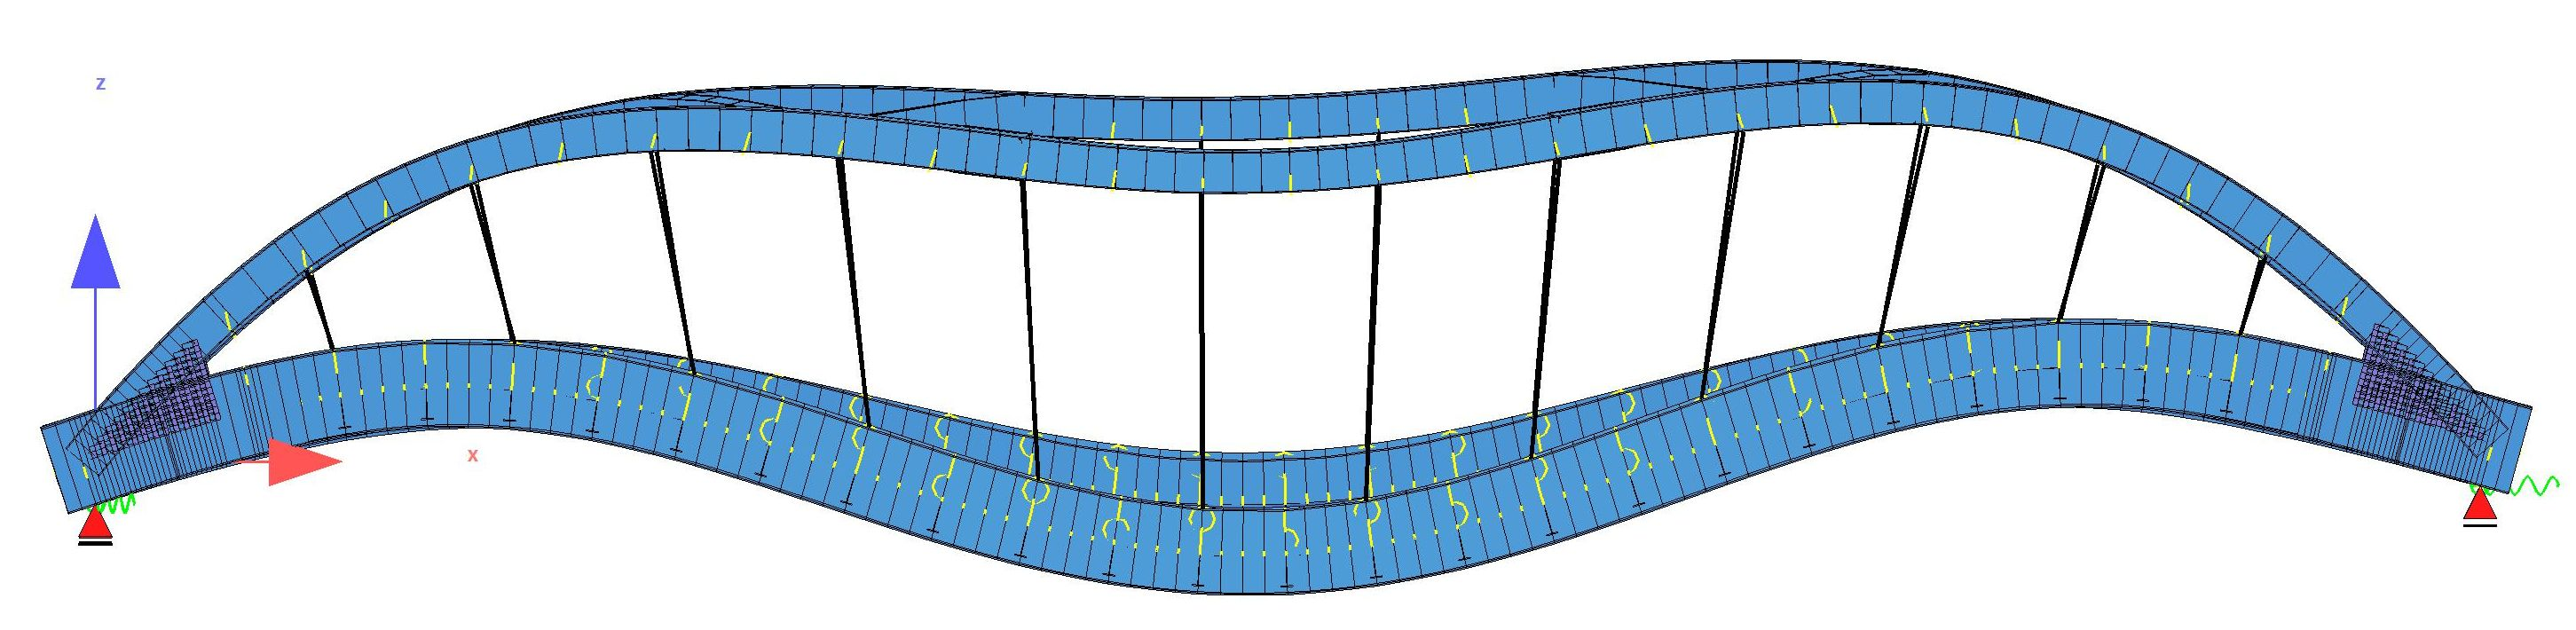
\includegraphics[width=0.7\textwidth]{/WK2/model/mod_origin/f7s.jpg}%
		\end{tabular}}\\
		\subfloat[Mod 8, $f_8=5.874 \text{ Hz}$]{\label{fig: wk2_origin_mod08}%
			\begin{tabular}[b]{c c}
				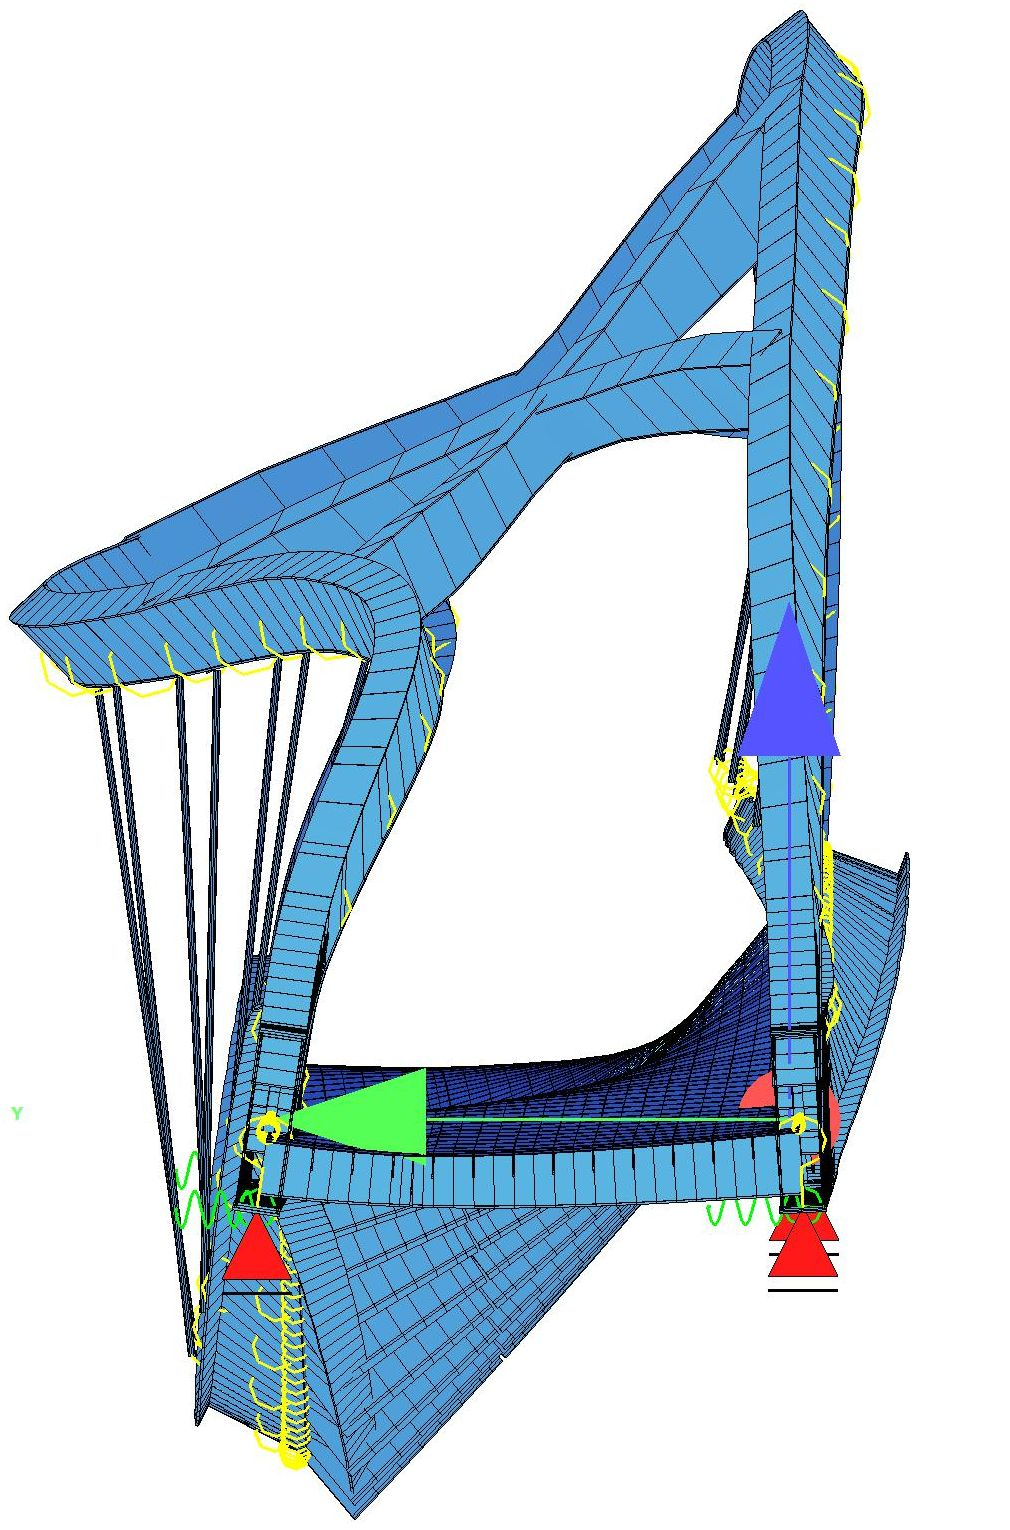
\includegraphics[height=0.12\textheight]{/WK2/model/mod_origin/f8f.jpg}%
				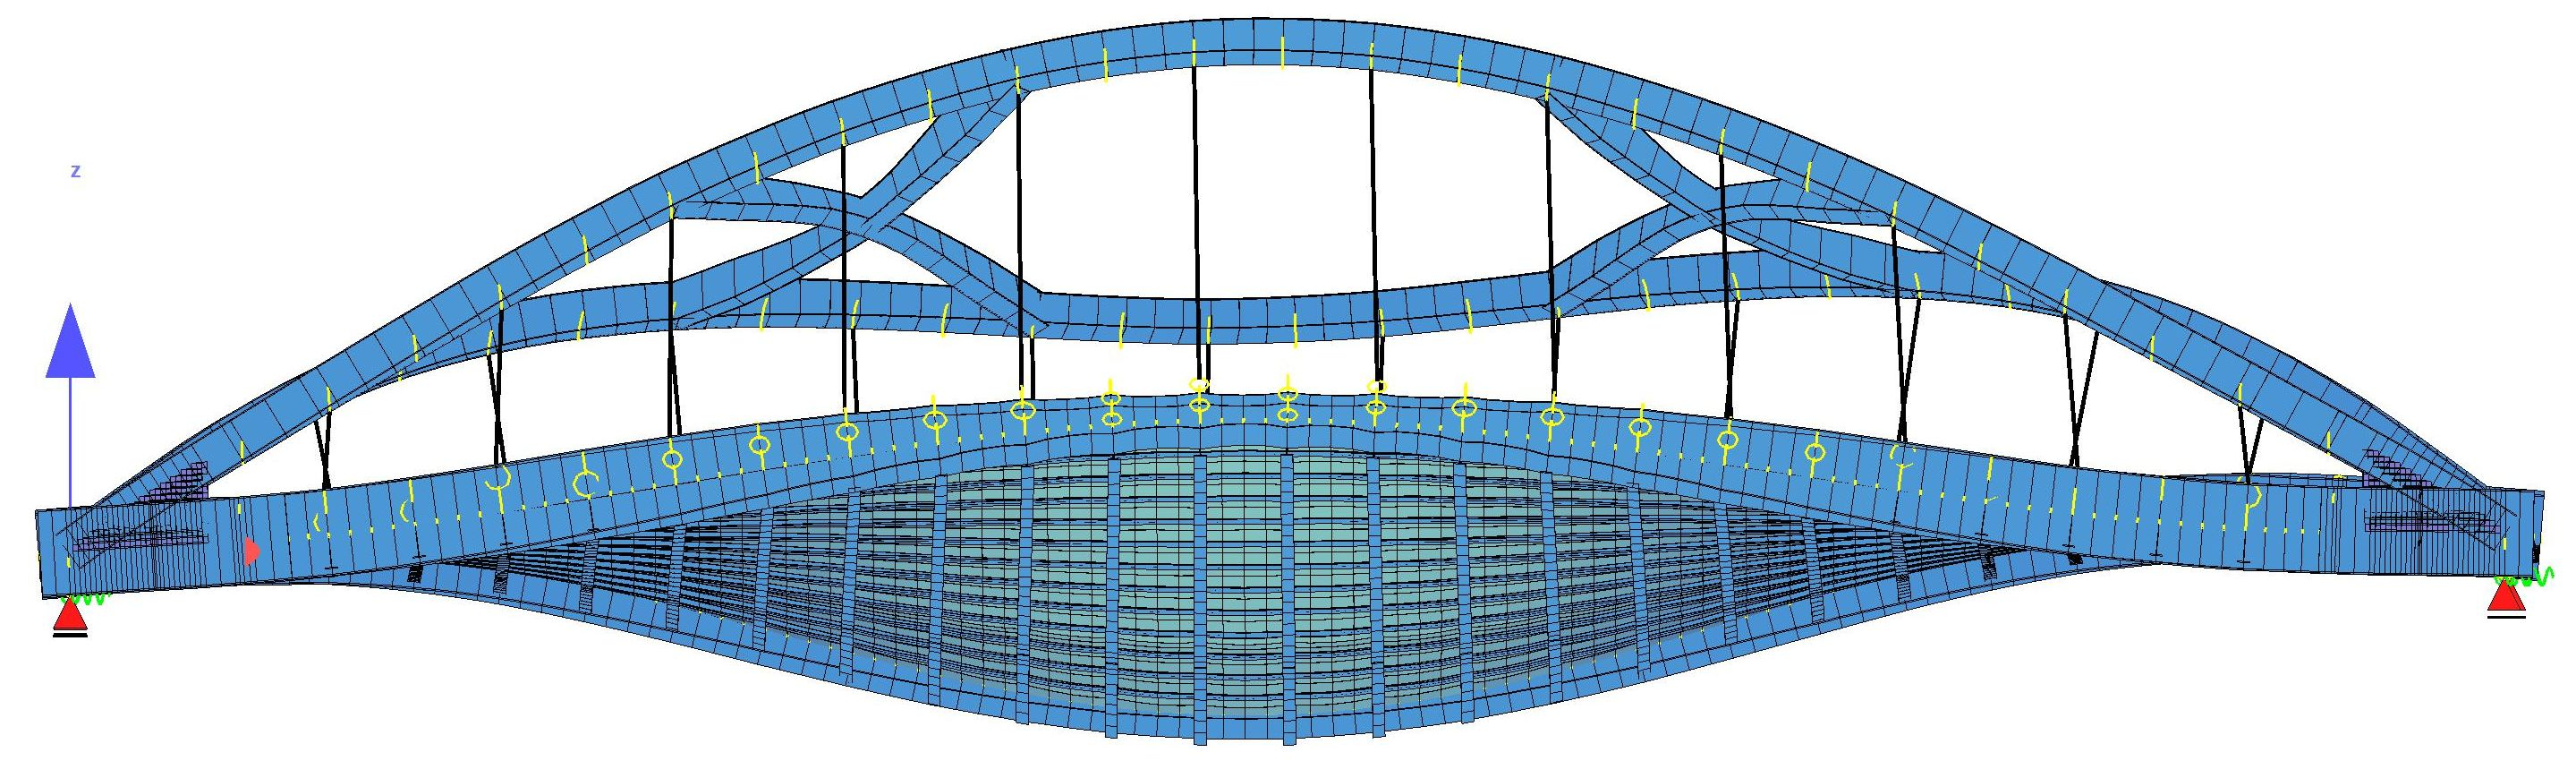
\includegraphics[width=0.7\textwidth]{/WK2/model/mod_origin/f8s.jpg}%
		\end{tabular}}\\
		\subfloat[Mod 9, $f_9=6.064 \text{ Hz}$]{\label{fig: wk2_origin_mod09}%
			\begin{tabular}[b]{c c}
				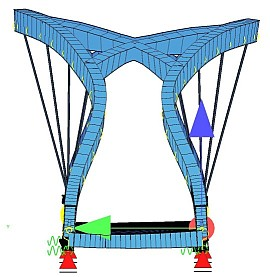
\includegraphics[height=0.12\textheight]{/WK2/model/mod_origin/f9f.jpg}%
				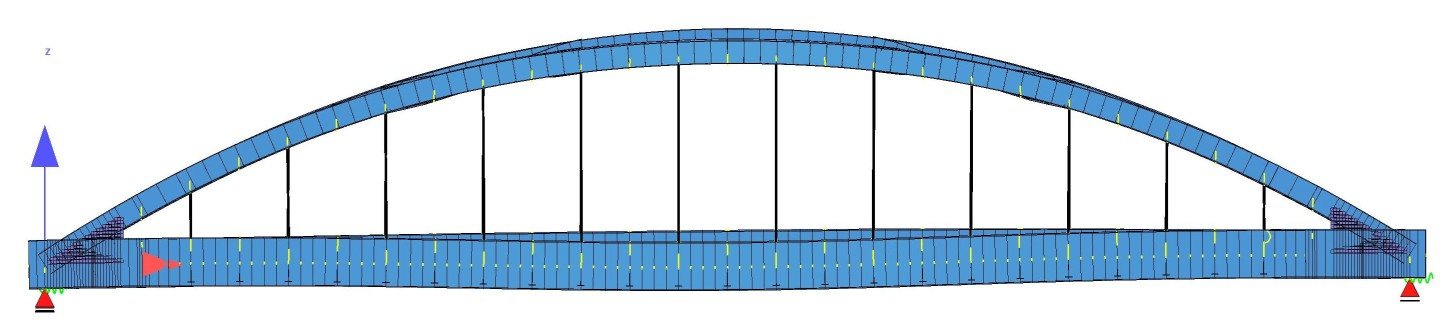
\includegraphics[width=0.7\textwidth]{/WK2/model/mod_origin/f9s.jpg}%
		\end{tabular}}\\
		\subfloat[Mod 10, $f_{10}=7.860 \text{ Hz}$]{\label{fig: wk2_origin_mod10}%
			\begin{tabular}[b]{c c}
				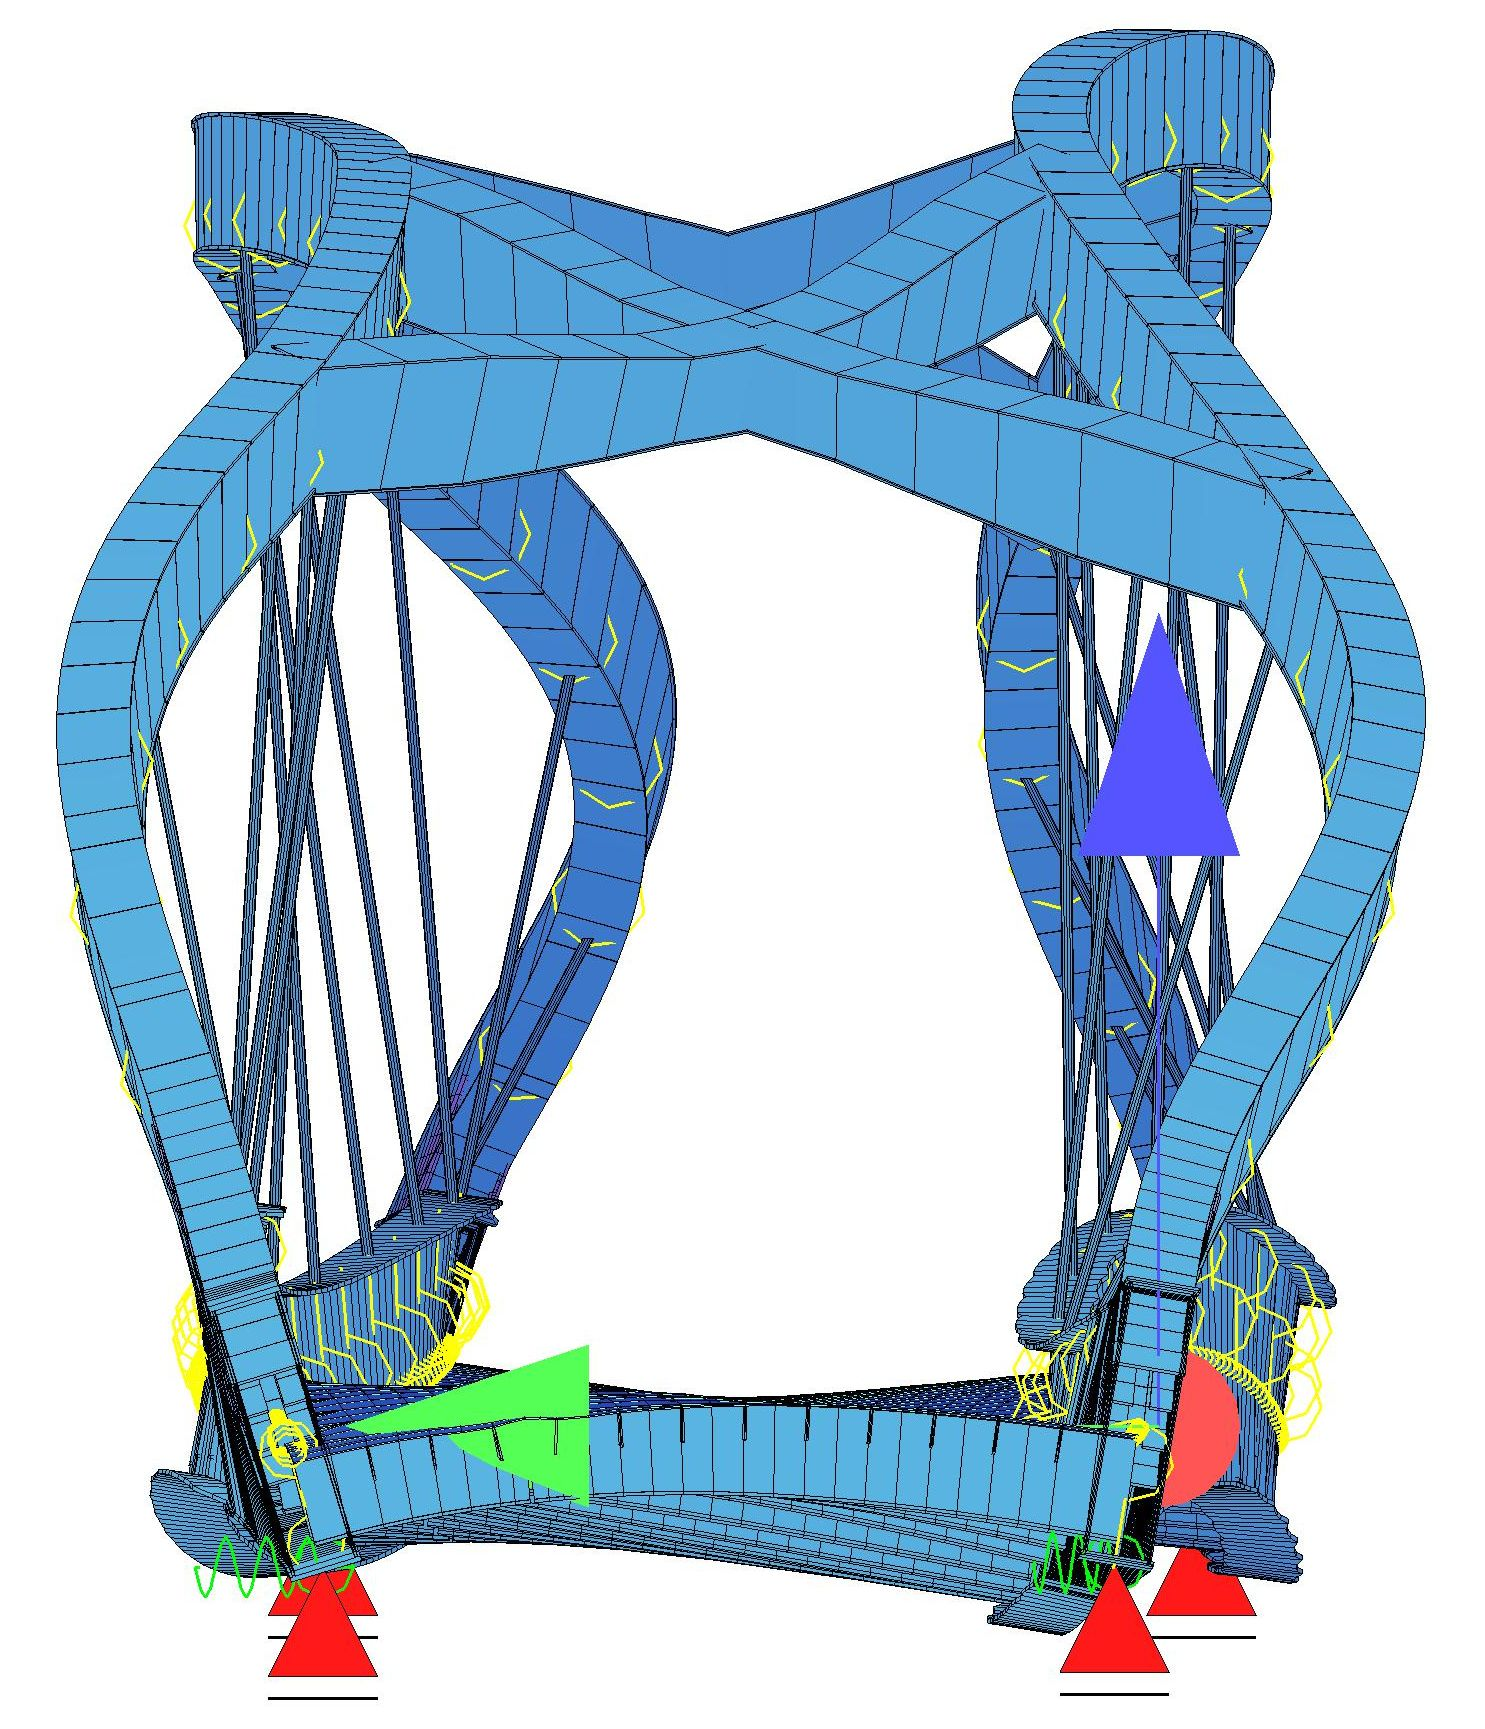
\includegraphics[height=0.12\textheight]{/WK2/model/mod_origin/f10f.jpg}%
				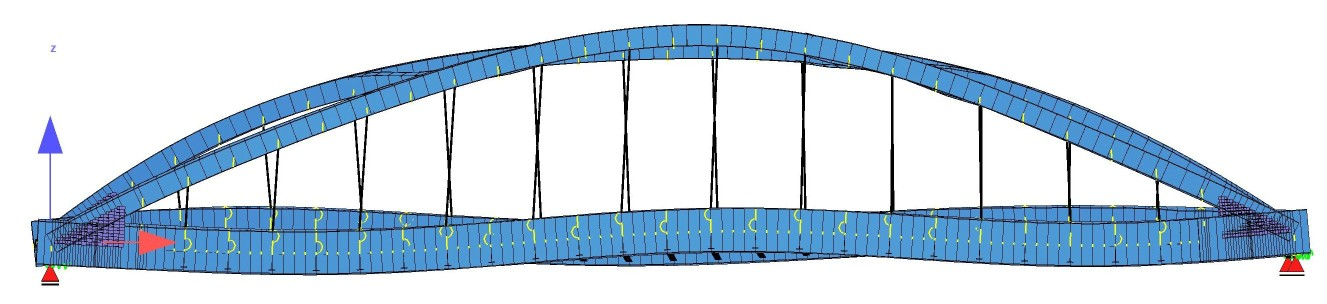
\includegraphics[width=0.7\textwidth]{/WK2/model/mod_origin/f10s.jpg}%
		\end{tabular}}\\
	\end{tabular}
	\caption{Postaci i częstotliwości drgań własnych wiaduktu WK2 - Model wstępny. Kont.}
	
\end{figure}

\section{Identyfikacja modalna wiaduktu WK2} \label{sect: identyfikacja_modalna_wk2}
Przed przystąpieniem do procesu optymalizacji układu statycznego dźwigara łukowego model należało skalibrować. Z uwagi na zakres planowanych analiz kluczowe dla analizy dynamicznej jest aby model w odpowiedni sposób odzwierciedlał rzeczywistość w zakresie parametrów modalnych. Mając do dyspozycji rzeczywisty obiekt, zdecydowano o wykonaniu badań terenowych, które pozwolą na identyfikację częstotliwości i postaci drgań własnych oraz towarzyszącego im tłumienia. Obiekt jest w ciągłej eksploatacji. Z tych względów zdecydowano o wykorzystaniu Operacyjnej Analizy Modalnej do identyfikacji parametrów modalnych przęsła.
Przed przystąpieniem do badań przygotowano plan zawierający kluczowe punkty, bez których spełnienia badania mogą zakończyć się niepowodzeniem lub wyniki mogą być trudne w interpretacji. \cite{Brincker2015} sporządzili listę zaleceń, które należy wypełnić w trakcie przygotowań eksperymentu OMA aby zakończył się on powodzeniem. Podobne zalecenia w swojej pracy sformułował \cite{Poprawa2018}. W kontekście założonych celów i wybranego obiektu badawczego główne z nich to:
\begin{itemize}[noitemsep]
\item opracowanie strategi prowadzenia badań i akwizycji danych,
\item uzgodnienia administracyjne - wstęp na obiekt i możliwość prowadzenia badań pod ruchem,
\item dobranie sprzętu pomiarowego.
\end{itemize}

Zarządca obiektu zezwolił na prowadzenie badań pod ruchem w towarzystwie sygnalisty. Średnie natężenie ruchu na obiekcie w trakcie badań to około 1 przejazd na 30 min. Wybór sprzętu pomiarowego ograniczał się do zastosowania posiadanego sprzętu do akwizycji przyspieszeń opisanego w punkcie (!!!). Najistotniejszym punktem przygotowania badań było opracowanie strategii badań. Według \cite{Brincker2015} plan badań OMA powinien zawierać następujące punkty:
\begin{itemize}[noitemsep]
	\item sporządzoną siatkę pomiarową,
	\item kolejność ustawień czujników w seriach pomiarowych,
	\item określenie liczby osób potrzebnych do przeprowadzenia eksperymentu,
	\item zapewnienie bezpieczeństwa w trakcie badań,
	\item określenie parametrów akwizycji danych (częstotliwość próbkowania, długość pomiarów, liczba powtórzeń serii pomiarowych itd.)
\end{itemize}

\subsubsection{Wybór punktów pomiarowych} \label{sect:choose_measuremanet_locations}
Dostępny system pomiarowy składał się z dwóch akcelerometrów 3-osiowych i z dwóch czujników 1-osiowych.  Mając do dyspozycji ograniczoną liczbę jednocześnie mierzonych punktów należało przeprowadzić symulację najlepszego rozmieszczenia punktów pomiarowych na obiekcie. Przykłady metod pozwalających na optymalne rozmieszczenie punktów pomiarowych w analizach dynamicznych zaprezentowano w literaturze i najczęściej opierają się one na wyznaczeniu reprezentatywnego wskaźnika, dzięki któremu da się porównać różne ustawienia. Między innymi \cite{Kammer1991,Papadopoulos1998} zaproponowali użycie Modalnej Energii Kinetycznej \teng{Modal Kinetic Energy}, \cite{Udwadia1994} macierzy informacyjnej Fishera \teng{Fisher Information Matrix}, a \cite{Penny1994,Allemang2003} macierzy MAC dla zestawu modów. \cite{Zhang2017} przedstawili zwięzłe zestawienie powyższych metod i zaproponowali opcję optymalizującą lokalizację punktów pomiarowych przy wielu ustawieniach pomiarowych, zarówno dla punktów pomiarowych jak i punktów referencyjnych. Autorzy zwracają również uwagę, że przy wielu punktach pomiaru ścisła ocena wszystkich możliwych ustawień jest wymagająca obliczeniowo bądź niemożliwa. Z tego względu stosowane są algorytmy heurystyczne bądź meta-heurystyczne. 

W niniejszej pracy zastosowano metodę wykorzystującą kryterium MAC \parencite{Penny1994}. Podobne postępowanie przedstawił w swojej pracy \cite{Poprawa2018}. Polega ono na wyznaczeniu teoretycznych postaci drgań własnych z dostępnego modelu MES. Dla zbioru wszystkich możliwych położeń czujników odczytywane są przemieszczenia znormalizowane danej postaci drgań. Ze zbioru możliwych położeń wybierane są punkty, gdzie umieszczone mają zostać czujniki. Posiłkując się opisem postaci drgań w wybranych punktach tworzona jest macierz MAC. Każdą postać porównuje się ze wszystkimi innymi i z samą sobą. W ten sposób na przekątnej macierzy pojawiają się wartości równe 1 co oznacza oczywiste, idealne dopasowanie według kryterium MAC dla równych wektorów. Poza przekątną, wartości MAC mieszczą się w przedziale 0 - 1. Celem analizy jest dobór punktów pomiarowych tak by poza przekątną wartości były możliwie małe. Przy małym dopasowaniu, postaci będą miały szanse być zidentyfikowane jednoznacznie przy mocno ograniczonej liczbie punktów pomiarowych i bliskim położeniu modów w dziedzinie częstotliwości. Dla każdego rozwiązania należy wyznaczyć wskaźnik, który pozwala ocenić zbiór punktów względem innych. \cite{Penny1994} zaproponowali w jednym z wariantów maksymalną wartość MAC wśród elementów poza przekątną macierzy oraz średnią kwadratową (RMS)\footnote{Średnią kwadratową wyznaczono zgodnie z definicją z równania: $x_{\text{RMS}}=\sqrt{\frac{x_1^2+x_2^2+x_3^2+\dots+x_n^2}{n}}$} ze wszystkich elementów powyżej przekątnej macierzy MAC. Im niższa wartość maksymalna i im niższa średnia kwadratowa tym lepiej.
\begin{figure}[t]
	\centering
	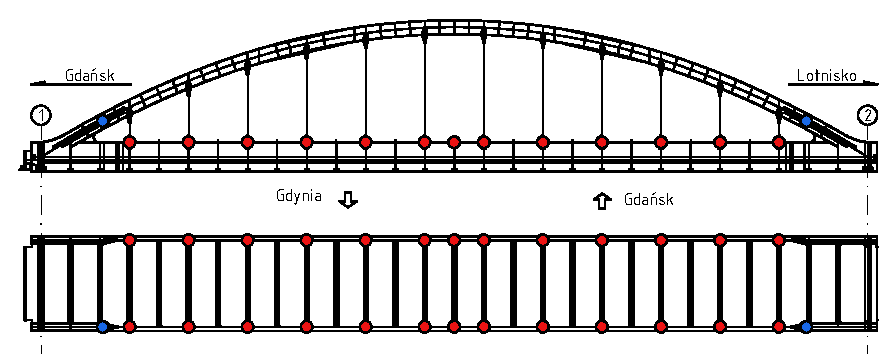
\includegraphics{/WK2/rysunki/punkty_pomiarowe_automac_croped.pdf}
	\captionsetup{justification=centering}
	\caption{Lokalizacje dozwolone przy doborze punktów pomiarowych}
	\label{fig: wk2_automac_points_all}
\end{figure}

Z uwagi na ograniczony czas dostępu do obiektu ustalono, że całość badań musi być zrealizowana w 3 ustawieniach dostępnych czujników. W przypadku wiaduktu, akcelerometry 3-osiowe potraktowano jako 2-osiowe. Odrzucono pomiar wzdłuż osi podłużnej obiektu jako nieistotny. W tej sytuacji jeden czujnik 2-osiowy posłużył jako punkt referencyjny mierzący drgania pionowe i poprzeczne. Pozostałe 4 punkty pomiarowe mogły być zmieniane w poszczególnych ustawieniach. Ostatecznie przy trzech ustawieniach możliwy był pomiar w 14 punktach pomiarowych $(6+4+4)$ w tym 10 na kierunku pionowym $Z$ i 4 na kierunku poprzecznym $Y$. Kolejnym koniecznym przy doborze siatki pomiarowej ograniczeniem było to, że dostęp do konstrukcji był możliwy jedynie z pomostu. Z uwagi na występowanie modów związanych głównie z bocznym ruchem łuków (rys. \ref{fig: model_wk2_origin_mods}) narzucono, że 4 punkty pomiarowe $2Y$ i $2Z$ zostaną zamocowane bezpośrednio na łuku. Uwzględniając powyższe założenia pozostało do dyspozycji 8 punktów pomiarowych $Z$ i 2 punkty pomiarowe $Y$. Punkty $Y$ są związane z $Z$ w ramach obudowy czujnika 2-osiowego, zaniechano więc doboru lokalizacji z uwagi na punkty $Y$ i skupiono się tylko na kierunku $Z$. Na rysunku \ref{fig: wk2_automac_points_all} kolorem czerwonym zaznaczono zbiór wszystkich dozwolonych do wyboru punktów. Kolorem niebieskim zaznaczono punkty zarezerwowane dla czujników mocowanych do łuku. Punków czerwonych jest 26 i należy z nich wybrać 8. Wykonano kombinację bez powtórzeń i uzyskano 1562275 zestawów lokalizacji czujników. Dla każdego zestawu wyznaczono macierz MAC uwzględniając 10 pierwszych modów z modelu MES, a następnie RMS i maksymalny element każdej macierzy. Zestawy posortowano względem każdego parametru i wyniki przedstawiono graficznie na rysunku \ref{fig: wk2_automac_charts}. 
\begin{figure}[t]
	\centering
	\captionsetup{justification=centering}
	\subfloat[Maksymalne MAC z elementów poza przekątną macierzy]{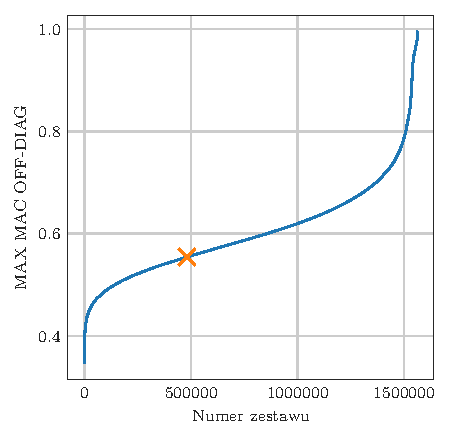
\includegraphics[]{/WK2/automac/max_mac.pdf}}% 
	\subfloat[RMS z elementów poza przekątną macierzy]{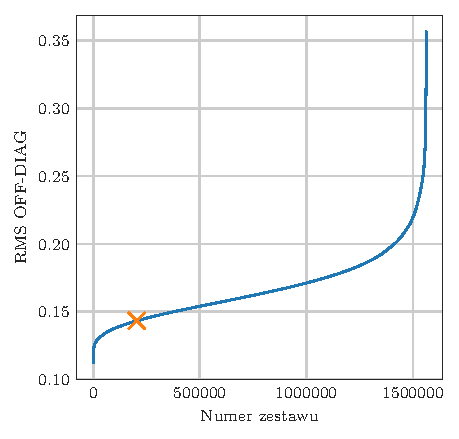
\includegraphics[]{/WK2/automac/rms.pdf}} 
	\captionsetup{justification=centering}
	\caption{Wskaźniki oceniające jakość wyboru zestawu punktów pomiarowych dla wszystkich analizowanych kombinacji}
	\label{fig: wk2_automac_charts}
\end{figure}
Logicznym wyborem punktów byłoby wzięcie pod uwagę ustawień charakteryzujących się minimalną wartością jednego z parametrów. Jednakże prowadząc badania terenowe należy brać pod uwagę czynniki takie jak ułożenie kabli, możliwości systemu pomiarowego do łączenia punktów pomiarowych, przejście przez czynną linię kolejową. Z tego powodu zaproponowano układ czujników intuicyjnie pozwalających na dobrą identyfikację modalną, a jednocześnie gwarantujący komfort w montażu i kontroli przez jedną osobę. Wybrane punkty pokazano na rysunku \ref{fig: wk2_automac_points_choosen}. Dla wybranego zestawu punktów wyznaczono macierz MAC (Rys. \ref{fig: wk2_automac_correlogram}) i wskaźniki: RMS i maksymalną wartość MAC. Wskaźniki zaznaczono na rysunku \ref{fig: wk2_automac_charts} pomarańczowym krzyżykiem, pokazując jakość dokonanego wyboru wśród wszystkich możliwych. Na podstawie wartości RMS można stwierdzić, że narzucony wariant charakteryzuje się niską wartością parametru i jego dalsze optymalizowanie kosztem utrudnień w trakcie pomiarów, oceniono jako nieopłacalne. Należy również zaznaczyć, że wartość RMS elementów poza przekątną macierzy MAC mierzy jedynie średnią zależność wszystkich par wektorów. Nie uwzględnia wielkości amplitud poszczególnych modów w punktach i ich znaczenia na ostateczne zachowanie dynamiczne kładki. W przedmiotowym przypadku zamocowano punkty pomiarowe w miejscach, gdzie kryterium RMS jest jednocześnie niskie (Rys. \ref{fig: wk2_automac_charts}) i przemieszczenia modalne dla głównych modów giętnych i skrętnych pomostu są bliskie ekstremalnym (Rys. \ref{fig: model_wk2_origin_mods}).




\begin{figure}[h]
	\centering
	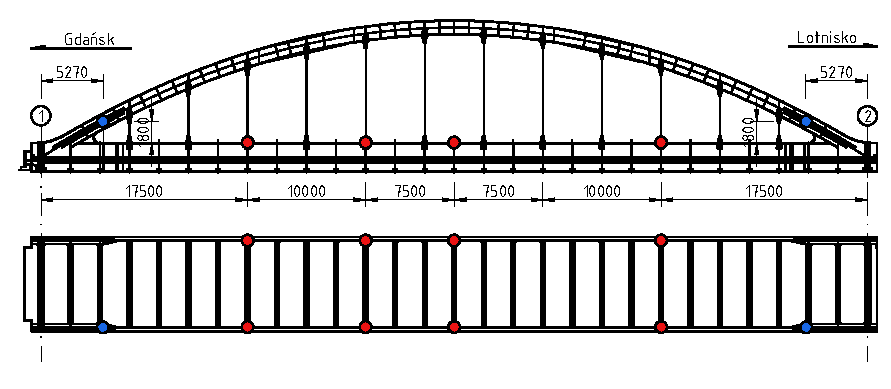
\includegraphics{/WK2/rysunki/punkty_pomiarowe_punkty_pomiarowe_croped.pdf}
	\captionsetup{justification=centering}
	\caption{Wybrane do badań punkty pomiarowe}
	\label{fig: wk2_automac_points_choosen}
\end{figure}





\begin{figure}[H]
	\centering
	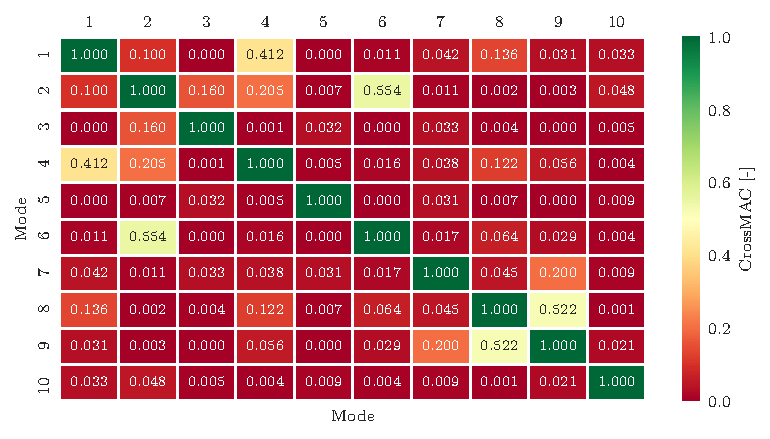
\includegraphics[width=\textwidth]{WK2/automac/correlogram_0.pdf}
	\captionsetup{justification=centering}
	\caption{Macierz MAC dla pierwszych dziesięciu wektorów postaci drgań własnych, odczytanych z modelu dla wybranych punktów pomiarowych}
	\label{fig: wk2_automac_correlogram}
\end{figure}


\subsubsection{Parametry akwizycji danych}
Przed przystąpieniem do badań wyznaczono podstawowe parametry pozwalające na przeprowadzenie poprawnego eksperymentu OMA. Posługując się formułami (\ref{eq: oma_min_sampling} - \ref{eq: oma_min_sampling}) określono minimalną częstotliwość próbkowania jako $f_{s,min}=2.4\cdot8=19.2\text{Hz}$ i minimalny czas prowadzenia pomiarów w jednym ustawieniu jako $T_{min}=\frac{10}{0.005\cdot1.4}=1429\text{s}=23.8\text{min}$. Ostatecznie zdecydowano o prowadzeniu pomiarów ze znacznym nadpróbkowaniem o częstotliwości $f_s=300\text{Hz}$ i w seriach czasowych 20 do 30 min.


\subsubsection{Przebieg badań}
Badania na obiekcie przeprowadzone zostały w dniu 17 czerwca 2019 r. Wykorzystano zestaw pomiarowy opisany w rozdziale \ref{sect: next_era_lab_test}. Zestaw w trakcie badań pokazano na rysunku \ref{fig: wk2_foto_aparatura}. Pomiary wykonano zgodnie z planem. Akwizycję danych podzielono na 3 ustawienia. Akwizycja danych w każdym ustawieniu wynosiła od 20 do 30 min. Punkty pomiarowe w poszczególnych ustawieniach oznaczono na rysunku \ref{fig: wk2_automac_points_choosen}. Warunki atmosferyczne były stabilne: brak odczuwalnych podmuchów wiatru, silne operowanie słońca.

\subsubsection{Środki obciążeniowe}
W trakcie badań na obiekcie odbywał się standardowy dla PKM ruch pociągów pasażerskich. Pomiędzy przejazdami, w asyście sygnalisty eksperymentator przemieszczał się biegając i podskakując po obiekcie. \ref{fig: wk2_foto_obciazenia}. Porównanie amplitud drgań bez wymuszenia i z dodatkowym wymuszeniem pokazano na rysunku \ref{RYSUNEK POMIAR DRGAN}. Z punktu widzenia pomiaru drgań środowiskowych należy zwrócić uwagę na pomniejsze oddziaływania występujące przy braku obciążeń kolejowych na obiekcie. Pod obiektem odbywał się ruch w ciągu magistralnej linii kolejowej nr 202. W odległości około 150 m od wiaduktu, niemal równolegle przebiega główna arteria Gdańska - aleja Grunwaldzka, na której ciągu dnia panuje stały, znaczny ruch samochodowy. W podobnej odległości od obiektu panowały prace budowlane z wykorzystaniem ciężkiego sprzętu.

\begin{figure}[h]
	\centering
	\subfloat[System akwizycji danych: komputer i wzmacniacz pomiarowy HBM PMX]{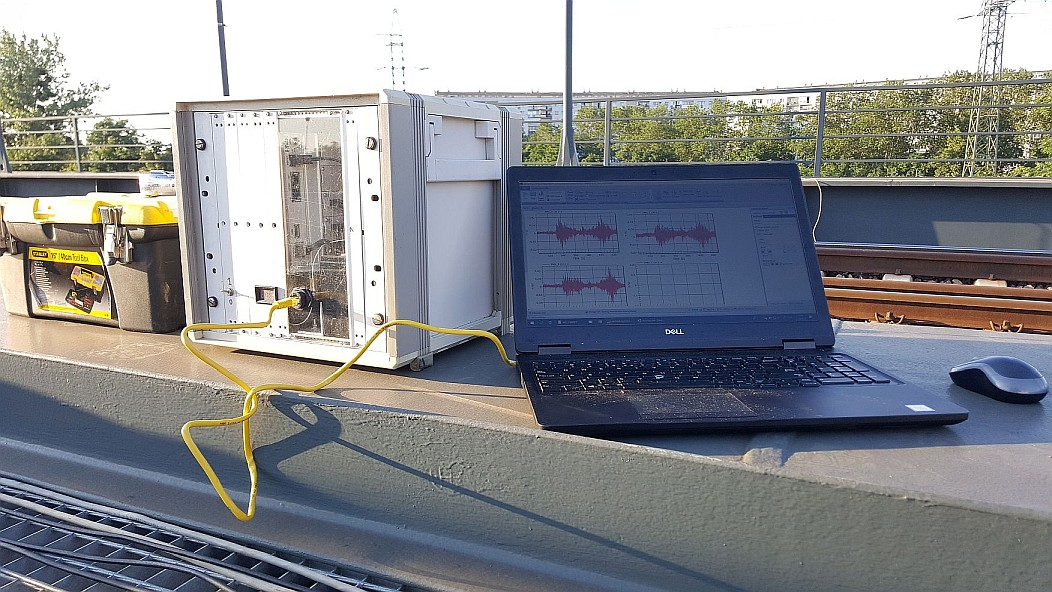
\includegraphics[width=0.48\linewidth]{/WK2/zdjecia/system_pomiarowy.jpg}} \quad 
	\subfloat[3 osiowy akcelerometr piezorezystancyjny]{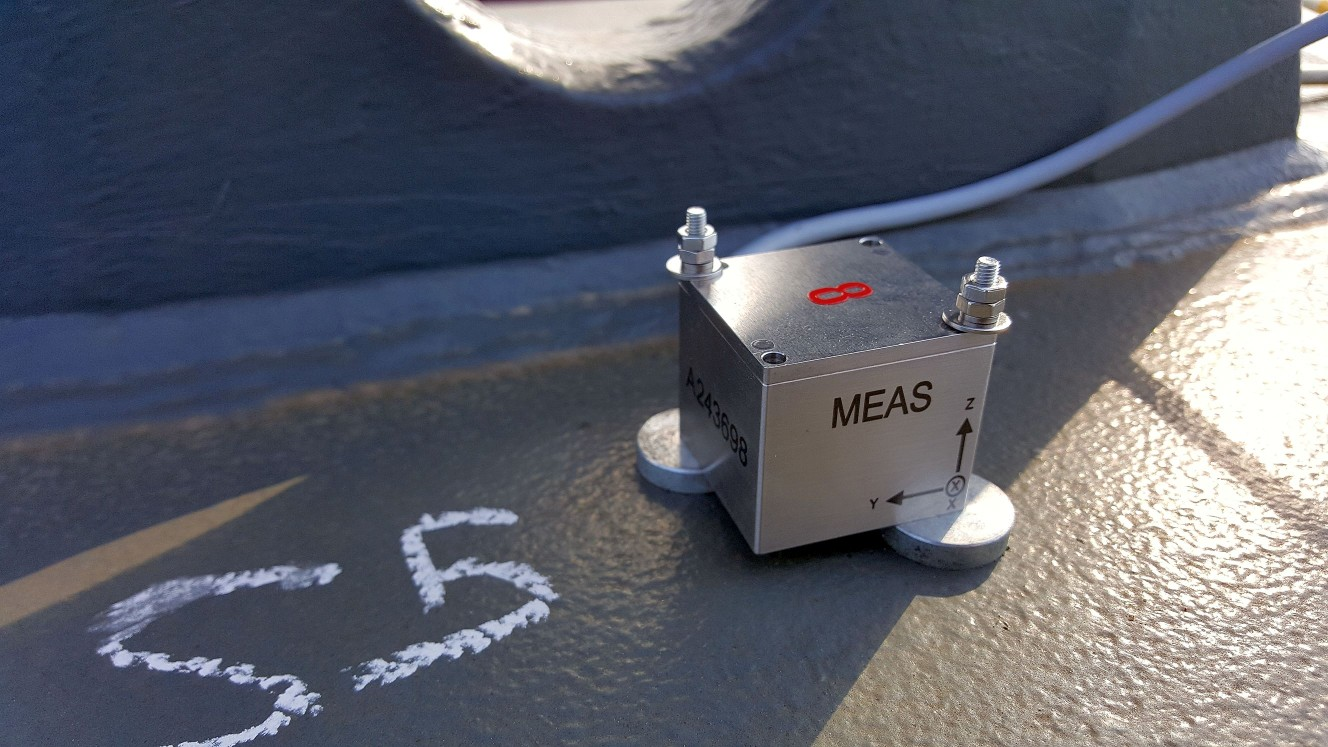
\includegraphics[width=0.48\linewidth]{/WK2/zdjecia/czujnik_3_osie.jpg}} 
	\captionsetup{justification=centering}
	\caption{System pomiarowy użyty do identyfikacji modalnej wiaduktu WK2}
	\label{fig: wk2_foto_aparatura}
\end{figure}

\begin{figure}[h]
	\centering
	%\subfloat[]{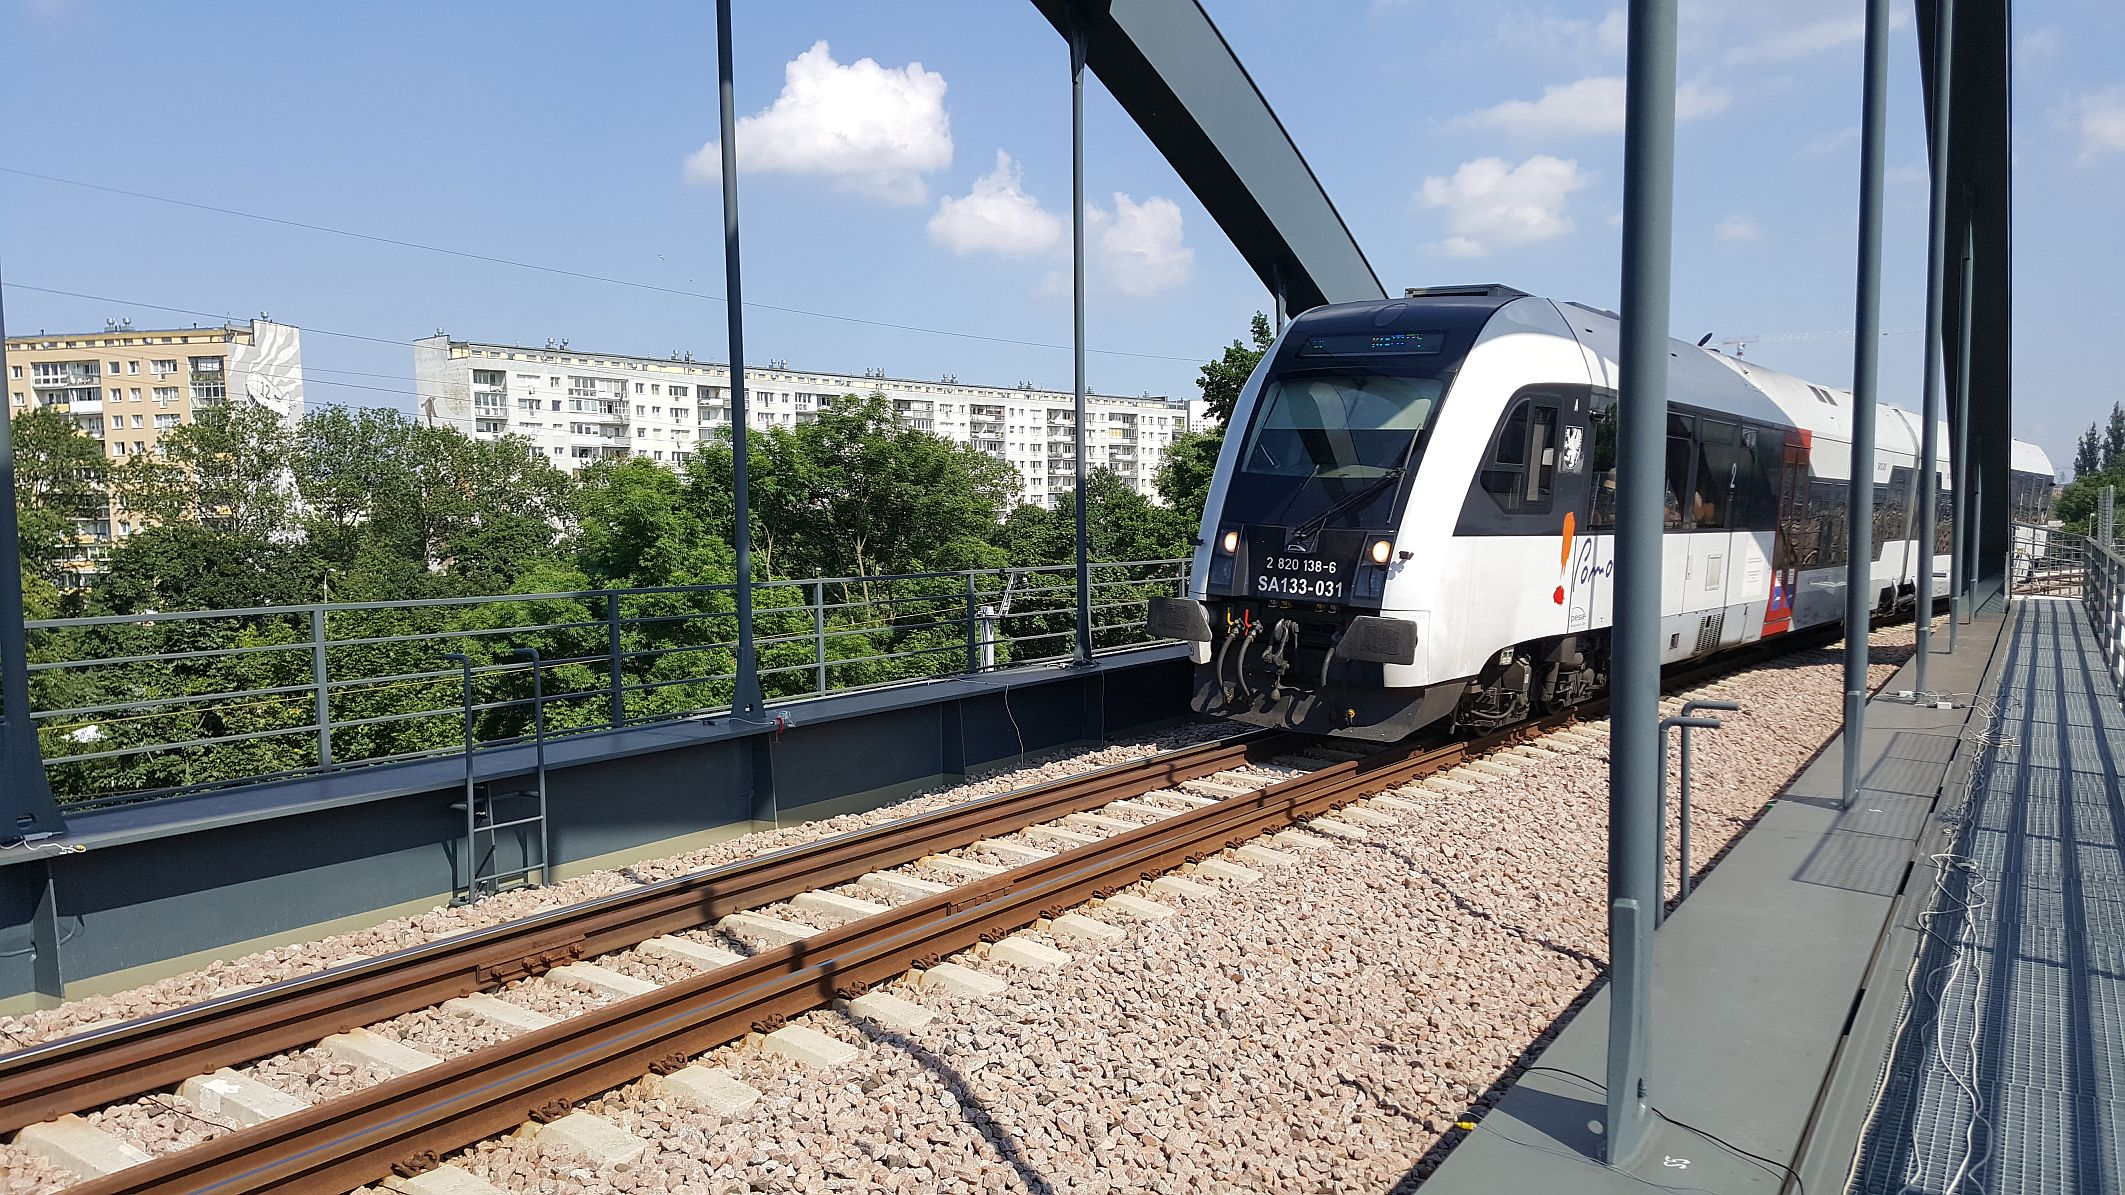
\includegraphics[height=0.15\textheight]{/WK2/zdjecia/pojazd_na.jpg}} \quad
	%\subfloat[]{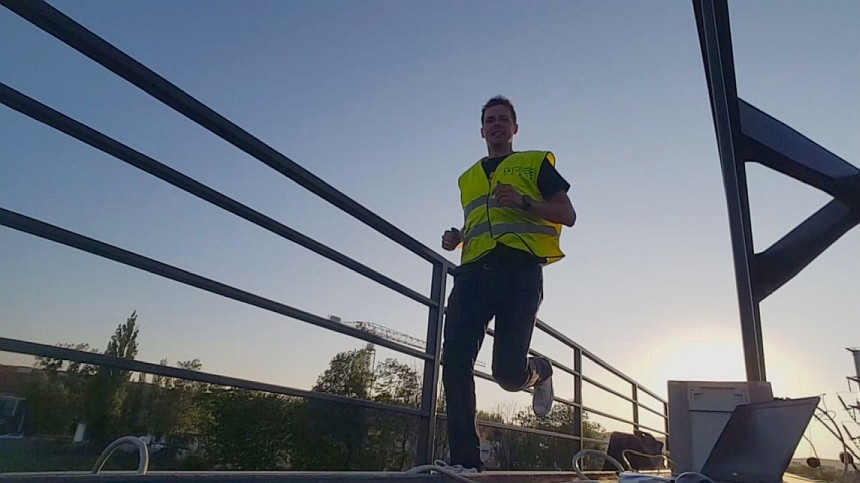
\includegraphics[height=0.15\textheight]{/WK2/zdjecia/eksperymentator.jpg}}
	\subfloat[Pojazd SA133-031 wjeżdżający na obiekt]{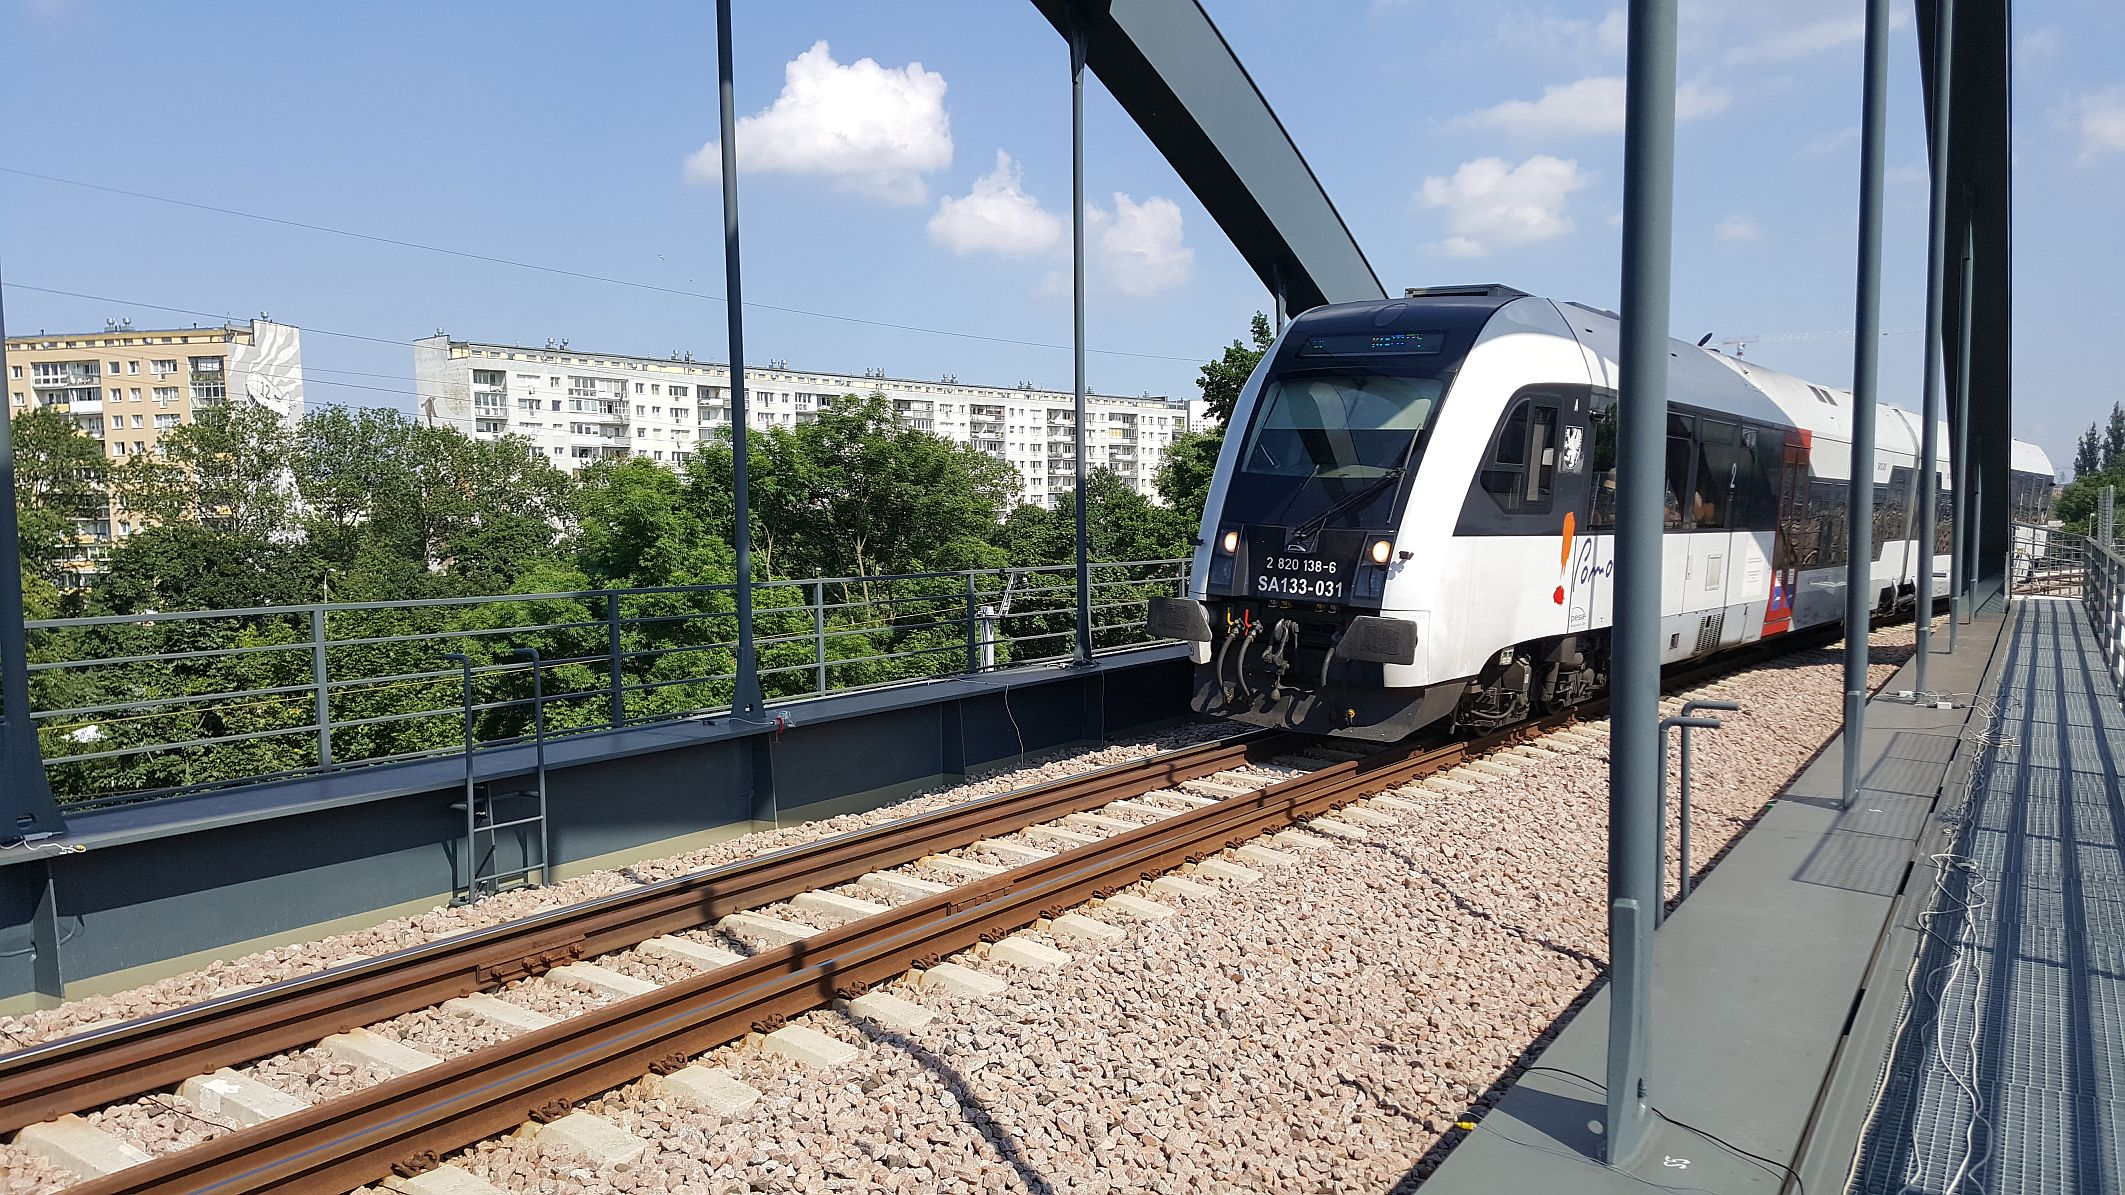
\includegraphics[width=0.48\textwidth]{/WK2/zdjecia/pojazd_na.jpg}} \quad
	\subfloat[Eksperymentator poruszający się po obiekcie]{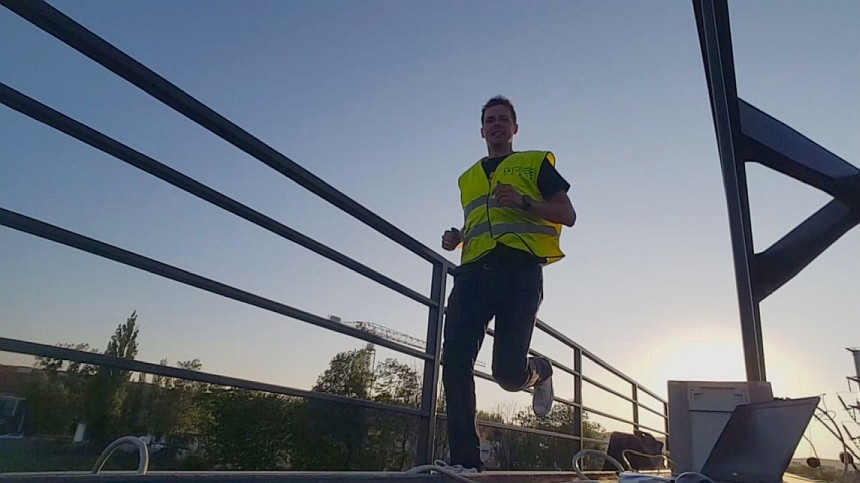
\includegraphics[width=0.48\textwidth]{/WK2/zdjecia/eksperymentator.jpg}}
	\captionsetup{justification=centering}
	\caption{Obciążenia w trakcie badań obiektu WK-2}
	\label{fig: wk2_foto_obciazenia}
\end{figure}

\subsubsection{Analiza i rezultaty badań}
Zarejestrowane sygnały poddano analizie OMA metodą NExT-ERA. W procesie iteracyjnym przyjęto parametry metody pozwalające uzyskać stabilne rozwiązania. Uwzględniając wyniki z analizy modalnej modelu teoretycznego (rys. \ref{fig: model_wk2_origin_mods}), stwierdzono że niektóre częstotliwości drgań własnych są bardzo bliskie. \cite{Caicedo2011} w takiej sytuacji proponuje obniżenie częstotliwości próbkowania sygnału. Zabieg ten zwiększa szanse na zidentyfikowanie blisko położonych modów przez uwzględnienie w analizie mniejszego, całkowitego zakresu częstotliwości. Zastosowano resampling do próbkowania 30Hz. Szerokość okna FFT przy obliczaniu funkcji korelacji przyjęto jako 1024. Wybrane okno przy zmniejszonej częstotliwości próbkowania pozwoliło uzyskać funkcje korelacji o długości około 17s. Wymiary macierzy Hankela przyjęto jako $r=110$ i $s=150$. Uwzględniono w ten sposób w macierzy Hankela niespełna 9s odpowiedzi impulsowej konstrukcji danej funkcjami korelacji. Taki czas pozwala na uwzględnienie kilkunastu okresów drgań modu o najniższej częstotliwości. Na rysunku \ref{fig: wk2_research_stabdiags} przestawiono diagramy stabilizacyjne metody w wersji filtrowanej i niefiltrowanej dla rzędu maksymalnego równego $n=150$. Przy tworzeniu diagramów zastosowano następujące kryteria poprawności rozwiązania:
\begin{itemize}[noitemsep]
	\item maksymalna różnica częstotliwości (\ref{eq: stabdiag_crit_freq}): $\Delta f \le 0.005$,
	\item maksymalny tłumienia (\ref{eq: stabdiag_crit_ksi}): $\Delta \xi \le 0.03$,
	\item minimalne kryterium MAC i MPC (\ref{eq: stabdiag_crit_MPC_MAC}): $\text{MPC}\ge 0.95$ \quad$\text{MAC}\ge 0.95$
\end{itemize}


 Zidentyfikowano 10 pierwszych modów o częstotliwościach mniejszych niż 8 Hz. Pomimo zidentyfikowania również modów o wyższych częstotliwościach dalsze rozważania ograniczono do pierwszych dziesięciu. Z praktycznego punktu widzenia, dla obiektów mostowych jedynie kilka najniższych modów ma znaczący wpływ na odpowiedź dynamiczną konstrukcji. Charakterystyki zidentyfikowanych modów przedstawiono na wykresach \ref{fig: wk2_research_mods1} i w tabeli \ref{tab: wk2_ident_mods}. Pierwszych 10 zidentyfikowanych częstotliwości drgań własnych jest zbliżonych do wyznaczonych analitycznie ze wstępnego modelu MES (Rys. \ref{fig: model_wk2_origin_mods}). Wartości Logarytmicznego Dekrementu Tłumienia wahają się od 1.3\% do 7.7\%. Biorąc pod uwagę, że Wiadukt WK2 jest konstrukcją stalową z korytem wypełnionym podsypką, rezultaty te nie wzbudzają zastrzeżeń. Zidentyfikowane postaci drgań pozwalają odróżnić od siebie mody, ale wyraźnie cierpią z uwagi na zbyt słabe odwzorowanie postaci. Postaci związane z drganiami poprzecznymi łuków identyfikowane są przez węzły zlokalizowane blisko wezgłowii i przez przemieszczenia pomostu realizujące się przez połączenie łuków ze ściągiem za pomocą wieszaków. Pomimo wspólnej normalizacji przemieszczeń modalnych pionowych i poprzecznych, wartości dla punków na łukach nie są znacznie większe niż przemieszczenia pomostu. Utrudnia to jednoznaczne powiązanie dla bliskich sobie modów z postaciami uzyskanymi w modelu teoretycznym. Gdyby to było możliwe, zamocowanie punktów pomiarowych na łuku w większej liczbie i w wyższych partiach mogłoby istotnie ułatwić identyfikację postaci i dalsze działania związane z kalibracją modelu. Podsumowując, identyfikację uznano za udaną i pozwalającą na ocenę konstrukcji i kalibrację modelu numerycznego.

\begin{figure}[]
	\centering
	\subfloat[Diagram niefiltrowany]{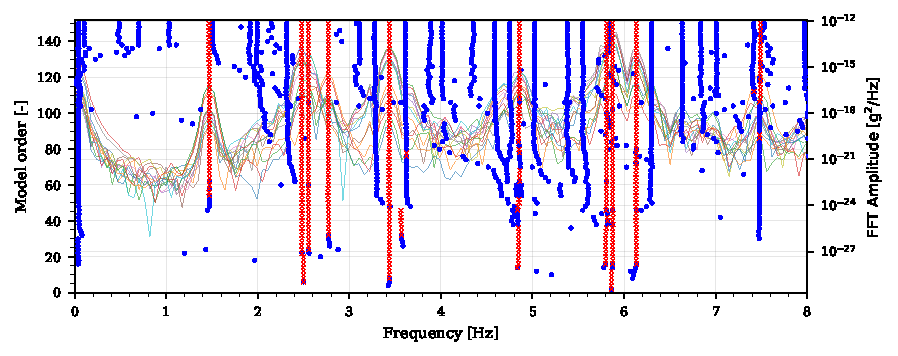
\includegraphics[]{WK2/ident/fig_stab_diagram_nonfiltr.pdf}}\\
	\subfloat[Diagram filtrowany]{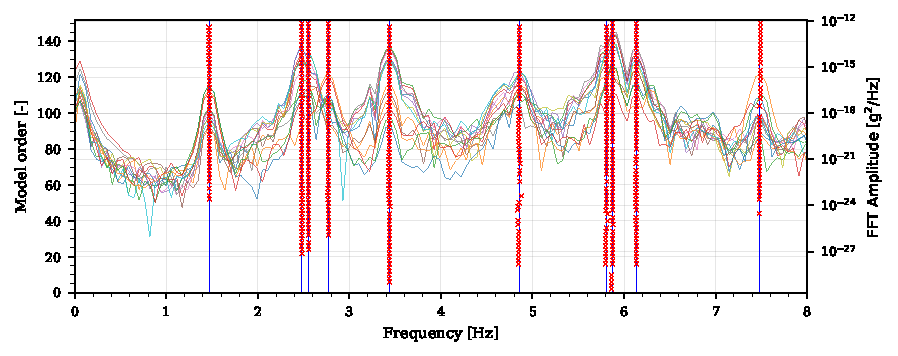
\includegraphics[]{WK2/ident/fig_stab_diagram_filtr.pdf}}
	\captionsetup{justification=centering}
	\caption{Diagramy stabilizacyjne metody NExT-ERA w badaniach wiaduktu WK2}
	\label{fig: wk2_research_stabdiags}
\end{figure}

\begin{table}[]
	\caption{Zidentyfikowane charakterystyki modalne wiaduktu WK2}
	\label{tab: wk2_ident_mods}
	\resizebox{\textwidth}{!}{%
	\begin{tabular}{@{}lcccccccccc@{}}
	\toprule
	\multicolumn{1}{c}{}              & \textbf{Mod 1} & \textbf{Mod 2} & \textbf{Mod 3} & \textbf{Mod 4} & \textbf{Mod 5} & \textbf{Mod 6} & \textbf{Mod 7} & \textbf{Mod 8} & \textbf{Mod 9} & \textbf{Mod 10} \\ \midrule
	\textbf{Częstotliwość {[}Hz{]}}   & 1.468          & 2.481          & 2.551          & 2.769          & 3.435          & 4.853          & 5.809          & 5.874          & 6.132          & 7.483           \\
	\textbf{Liczba tłumienia {[}-{]}} & 0.007          & 0.009          & 0.006          & 0.011          & 0.012          & 0.012          & 0.005          & 0.005          & 0.002          & 0.004           \\
	\textbf{LDT {[}-{]}}              & 0.043          & 0.053          & 0.037          & 0.070          & 0.077          & 0.077          & 0.028          & 0.031          & 0.013          & 0.024           \\ \bottomrule
\end{tabular}}
\end{table}





\begin{figure}[p]
	\centering
	\begin{tabular}[c]{c}
	\subfloat[Mod 1, $f_1=1.468 \text{Hz}$]{\label{fig: wk2_research_mod01}%
			\begin{tabular}[b]{c c c}
				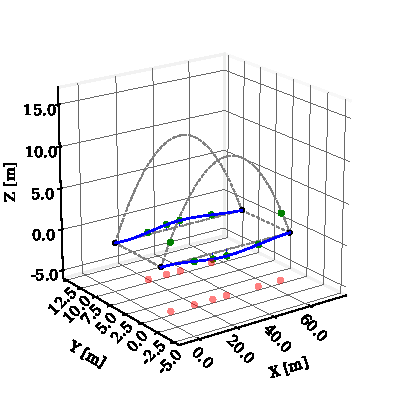
\includegraphics[height=0.20\textheight,trim=0 0 0 25,clip]{/wk2/ident/mods/fig_mod_11_time_20_08_21.pdf}%
				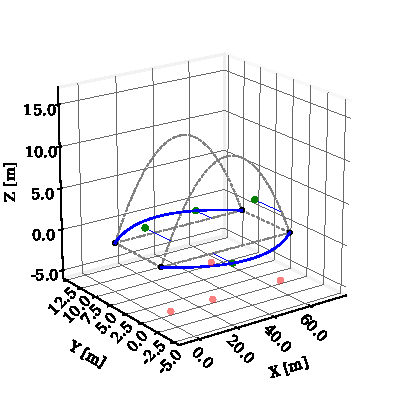
\includegraphics[height=0.20\textheight,trim=0 0 0 25,clip]{/wk2/ident/mods/fig_mod_11_time_20_09_01.pdf}%
				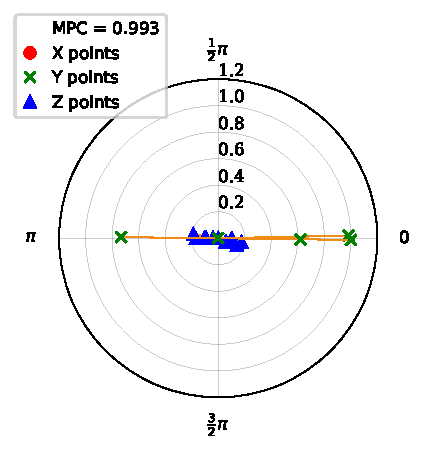
\includegraphics[height=0.20\textheight]{/wk2/ident/mods/fig_polar_mod_11_time_16_57_20.pdf}%
		\end{tabular}}\\
	\subfloat[Mod 2, $f_2=2.481 \text{Hz}$]{\label{fig: wk2_research_mod02}%
	\begin{tabular}[b]{c c c}
		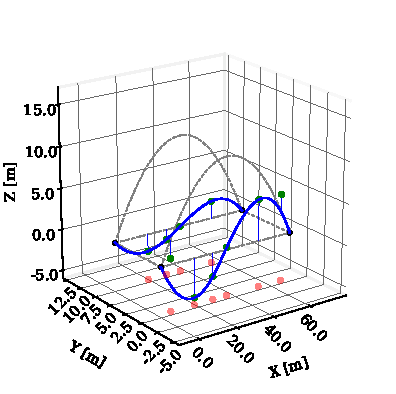
\includegraphics[height=0.20\textheight,trim=0 0 0 25,clip]{/wk2/ident/mods/fig_mod_23_time_20_09_19.pdf}%
		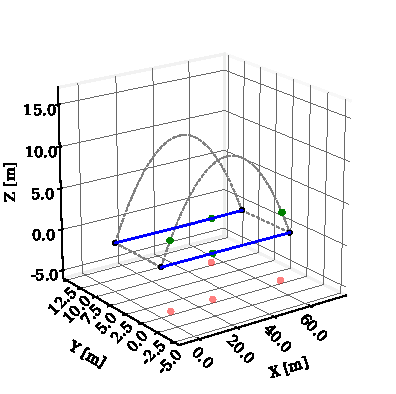
\includegraphics[height=0.20\textheight,trim=0 0 0 25,clip]{/wk2/ident/mods/fig_mod_23_time_20_09_26.pdf}%
		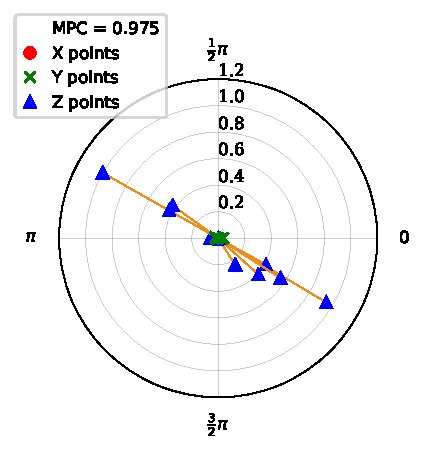
\includegraphics[height=0.20\textheight]{/wk2/ident/mods/fig_polar_mod_23_time_16_57_54.pdf}%
\end{tabular}}\\
	\subfloat[Mod 3, $f_3=2.551 \text{Hz}$]{\label{fig: wk2_research_mod03}%
	\begin{tabular}[b]{c c c}
		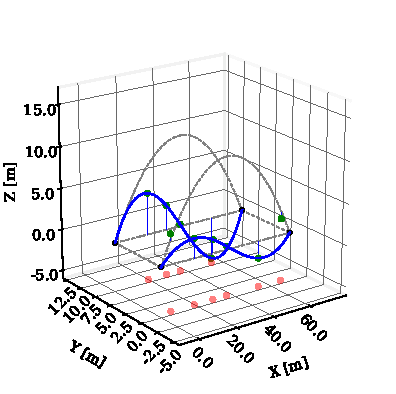
\includegraphics[height=0.20\textheight,trim=0 0 0 25,clip]{/wk2/ident/mods/fig_mod_25_time_20_09_56.pdf}%
		\includegraphics[height=0.20\textheight,trim=0 0 0 25,clip]{/wk2/ident/mods/fig_mod_25_time_20_10_13.pdf}%
		\includegraphics[height=0.20\textheight]{/wk2/ident/mods/fig_polar_mod_25_time_16_58_42.pdf}%
\end{tabular}}\\
	\subfloat[Mod 4, $f_4=2.769 \text{Hz}$]{\label{fig: wk2_research_mod04}%
	\begin{tabular}[b]{c c c}
		\includegraphics[height=0.20\textheight,trim=0 0 0 25,clip]{/wk2/ident/mods/fig_mod_27_time_20_10_31.pdf}%
		\includegraphics[height=0.20\textheight,trim=0 0 0 25,clip]{/wk2/ident/mods/fig_mod_27_time_20_10_46.pdf}%
		\includegraphics[height=0.20\textheight]{/wk2/ident/mods/fig_polar_mod_27_time_16_59_26.pdf}%
\end{tabular}}\\

	\end{tabular}
\caption{Zidentyfikowane charakterystyki modalne wiaduktu WK2}
\label{fig: wk2_research_mods1}
\end{figure}


\begin{figure}[p]\ContinuedFloat
	\centering
	\begin{tabular}[c]{c}
	\subfloat[Mod 5, $f_5=3.435 \text{Hz}$]{\label{fig: wk2_research_mod05}%
	\begin{tabular}[b]{c c c}
		\includegraphics[height=0.20\textheight,trim=0 0 0 25,clip]{/wk2/ident/mods/fig_mod_33_time_20_11_02.pdf}%
		\includegraphics[height=0.20\textheight,trim=0 0 0 25,clip]{/wk2/ident/mods/fig_mod_33_time_20_11_12.pdf}%
		\includegraphics[height=0.20\textheight]{/wk2/ident/mods/fig_polar_mod_33_time_17_00_05.pdf}%
\end{tabular}}\\

	\subfloat[Mod 6, $f_6=4.853 \text{Hz}$]{\label{fig: wk2_research_mod06}%
	\begin{tabular}[b]{c c c}
		\includegraphics[height=0.20\textheight,trim=0 0 0 25,clip]{/wk2/ident/mods/fig_mod_47_time_20_11_28.pdf}%
		\includegraphics[height=0.20\textheight,trim=0 0 0 25,clip]{/wk2/ident/mods/fig_mod_47_time_20_11_53.pdf}%
		\includegraphics[height=0.20\textheight]{/wk2/ident/mods/fig_polar_mod_47_time_17_00_46.pdf}%
\end{tabular}}\\
	\subfloat[Mod 7, $f_7=5.809 \text{Hz}$]{\label{fig: wk2_research_mod07}%
	\begin{tabular}[b]{c c c}
		\includegraphics[height=0.20\textheight,trim=0 0 0 25,clip]{/wk2/ident/mods/fig_mod_57_time_20_12_12.pdf}%
		\includegraphics[height=0.20\textheight,trim=0 0 0 25,clip]{/wk2/ident/mods/fig_mod_57_time_20_12_20.pdf}%
		\includegraphics[height=0.20\textheight]{/wk2/ident/mods/fig_polar_mod_57_time_17_01_27.pdf}%
\end{tabular}}\\
	\subfloat[Mod 8, $f_8=5.874 \text{Hz}$]{\label{fig: wk2_research_mod08}%
	\begin{tabular}[b]{c c c}
		\includegraphics[height=0.20\textheight,trim=0 0 0 25,clip]{/wk2/ident/mods/fig_mod_59_time_20_12_37.pdf}%
		\includegraphics[height=0.20\textheight,trim=0 0 0 25,clip]{/wk2/ident/mods/fig_mod_59_time_20_12_48.pdf}%
		\includegraphics[height=0.20\textheight]{/wk2/ident/mods/fig_polar_mod_59_time_17_02_08.pdf}%
\end{tabular}}\\
	\end{tabular}
\caption{Zidentyfikowane charakterystyki modalne wiaduktu WK2 kont.}
\label{fig: wk2_research_mods2}
\end{figure}


\begin{figure}[H]\ContinuedFloat
	\centering
	\begin{tabular}[c]{c}
	\subfloat[Mod 9, $f_9=6.132 \text{Hz}$]{\label{fig: wk2_research_mod09}%
	\begin{tabular}[b]{c c c}
		\includegraphics[height=0.20\textheight,trim=0 0 0 25,clip]{/wk2/ident/mods/fig_mod_61_time_20_13_07.pdf}%
		\includegraphics[height=0.20\textheight,trim=0 0 0 25,clip]{/wk2/ident/mods/fig_mod_61_time_20_13_32.pdf}%
		\includegraphics[height=0.20\textheight]{/wk2/ident/mods/fig_polar_mod_61_time_17_17_06.pdf}%
\end{tabular}}\\
	\subfloat[Mod 10, $f_{10}=7.483 \text{Hz}$]{\label{fig: wk2_research_mod10}%
	\begin{tabular}[b]{c c c}
		\includegraphics[height=0.20\textheight,trim=0 0 0 25,clip]{/wk2/ident/mods/fig_mod_75_time_20_13_51.pdf}%
		\includegraphics[height=0.20\textheight,trim=0 0 0 25,clip]{/wk2/ident/mods/fig_mod_75_time_20_14_02.pdf}%
		\includegraphics[height=0.20\textheight]{/wk2/ident/mods/fig_polar_mod_75_time_17_18_33.pdf}%
\end{tabular}}\\



	\end{tabular}
	\caption{Zidentyfikowane charakterystyki modalne wiaduktu WK2 kont.}
	\label{fig: wk2_research_mods3}
\end{figure}

\section{Kalibracja modelu numerycznego z wykorzystaniem PSO} \label{sect:wk2_calibration}
Stworzony model numeryczny powstał na podstawie założeń projektowych. Wykonana identyfikacja parametrów dynamicznych i przeprowadzone badania odbiorcze pod próbnym obciążeniem dostarczyły szereg informacji o obiekcie rzeczywistym. Dzięki dostarczonym danym możliwe jest przeprowadzenie kalibracji, która sprawi że model będzie wierniej odzwierciedlał rzeczywistą konstrukcję. Podsumowując wyznaczone i zdobyte wyniki, kalibracja opierać będzie się na następujących danych wyjściowych:
\begin{itemize}
	\item przemieszczenia statyczne konstrukcji pod próbnym obciążeniem: 2 ustawienia po 6 punktów pomiarowych umiejscowionyc na ściągach dźwigarów łukowych,
	\item zidentyfikowane parametry modalne konstrukcji: 10 pierwszych częstotliwości i postaci drgań własnych oraz odpowiadające im tłumienia modalne. Postaci drgań opisane zostały za pomocą 14 współrzędnych modalnych (p. \ref{sect:choose_measuremanet_locations})
\end{itemize}
Zestaw danych zmierzonych w ramach obciążeń statycznych pozwoli skalibrować głównie sztywność poszczególnych elementów konstrukcji. Z kolei parametry modalne, jako wartości odnoszące się do zachowania dynamicznego, związane są ze sztywnością konstrukcji, jak i masą konstrukcyjną i niekonstrukcyjną.
Obiekty łukowe, podobnie jak kratownicowe są relatywnie złożonymi obiektami. Na ich charakterystykę dynamiczną wpływa wiele czynników, które mniej lub bardziej potrafią wpłynąć na jego parametry. Różni to je od statycznie nieskomplikowanych obiektów belkowych czy płytowych oraz od dużych obiektów wiszących i podwieszonych gdzie rozwiązania i szczegóły konstrukcyjne nie wpływają aż tak istotnie na globalne zachowanie dynamiczne konstrukcji. Dla łukowego wiaduktu WK2 wyodrębniono 22 czynniki, które będą podlegać modyfikacji w trakcie kalibracji. Podzielono je na trzy rodzaje: sztywności elementów konstrukcyjnych, sztywności warunków brzegowych oraz masy konstrukcyjne i niekonstrukcyjne. Poniżej zestawiono symbole zmiennych wraz z ich opisem:
\begin{itemize}
	\item Sztywności elementów konstrukcyjnych:
	\begin{itemize}
		\item S1 - łuku,
		\item S2 - ściągu,
		\item S3 - poprzecznic,
		\item S4 - żeber płyty ortotropowej,
		\item S5 - blachy płyty ortotropowej,
		\item S6 - stężeń górnych,
		\item S7 - wieszaków,
		\item S8 - elementów stanowiących usztywniających wezgłowie łuku,  
	\end{itemize}
	\item Sztywność warunków brzegowych (Rys. \ref{fig:boudary_conditions_stiff_bearings}):
	\begin{itemize}
		\item S21 - Oś 2, podpora A, kierunek X,
		\item S22 - Oś 1, podpora A, kierunek Y,
		\item S23 - Oś 1, podpora B, kierunek X,
		\item S24 - Oś 2, podpora B, kierunek X,
		\item S25 - Oś 1, podpora A, kierunek X,
		\item S26 - Oś 2, podpora A, kierunek Y,
		\item S27 - Oś 1, podpora B, kierunek Y,
		\item S28 - Oś 2, podpora B, kierunek Y,
	\end{itemize}
	\item Masa elementów konstrukcyjnych i niekonstrukcyjnych:
	\begin{itemize}
		\item M1 - łuku,
		\item M2 - ściągu,
		\item M3 - tłucznia - część wzdłuż osi toru,
		\item M4 - tłucznia - część równomiernie rozłożona,
		\item M5 - pomostu roboczego,
		\item M6 - stężeń górnych.
	\end{itemize}
\end{itemize}

\begin{figure}[h]
	\centering
	\includegraphics[width=\textwidth]{WK2/rysunki/lozyska_sprezyny_kalibracja.pdf}
	\captionsetup{justification=centering}
	\caption{Schemat łożyskowania i rozmieszczenia podpór sprężystych, modyfikowanych w procesie kalibracji}
	\label{fig:boudary_conditions_stiff_bearings}
\end{figure}
Niektóre z wymienionych elementów intuicyjnie nie wpływają znacząca na globalne charakterystyki modalne konstrukcji. Dotyczy to między innymi sztywności elementów pomostu czy warunków brzegowych w przypadku zastosowania łożysk mostowych. Zostały one jednak uwzględnione w niniejszej pracy jako zmienne, żeby mieć pełną kontrolę nad modyfikacjami modelu oraz żeby uwidocznić zalety zastosowanej metody kalibracji.

Kalibrację modelu postanowiono potraktować jako problem optymalizacji. Problem zdefiniowano klasycznie przez wybór funkcji celu, parametrów i zmiennych projektowych oraz ograniczeń. Funkcją celu jest miara dopasowania modelu do konstrukcji rzeczywistej pod względem odpowiedzi statycznej i charakterystyk dynamicznych. Parametry projektowe definiują model numeryczny poddawany kalibracji i zostały przyjęte na podstawie dokumentacji powykonawczej. Zmienne projektowe stanowią wymienione wyżej 22 parametry: sztywności elementów konstrukcji, warunków brzegowych i masy znajdujące się na obiekcie.  Jako metodę optymalizacji przyjęto metodę roju cząstek PSO. 

\subsection{Funkcja celu}
Funkcja celu w zdefiniowanym problemie w założeniu miała być miarą dopasowania. W literaturze do kalibracji naczęściej stosowane są jednokryterialne algorytmy, w których miara dopasowania musi być wyrażona jedną liczbą. Wynikowa wartość jest więc najczęściej liniową kombinacją wag i kryteriów dopasowania. Chcąc uniknąć narzucania skali ważności na poszczególne kryteria, optymalizację wykonano w wariancie wielokryterialnym. Zbiorem funkcji celu, z których każda jest minimalizowana i opisuje dopasowanie modelu do obiektu jest wektor $\vect{F}=[f_{freq},f_{disp},f_{MAC}]$. Na wartość funkcji $f_{freq}$ wpływ ma $N$ pierwszych częstotliwości drgań własnych modelu $f_i^n$ i zidentyfikowanych na konstrukcji rzeczywistej $f_i^r$. Wyznaczana jest ona następująco:
\begin{equation} \label{eq:wk2_calib_f_freq}
f_{freq}=\sum_{i=1}^{N} (f_i^n - f_i^r)^2
\end{equation}
Funkcja celu $f_{disp}$ związana jest z przemieszczeniami uzyskiwanymi pod działaniem obciążenia statycznego. W rozważanym przypadku wykorzystano pomiar wykonany w trakcie próbnego obciążenia. Dla dwóch ustawień, po sześć punktów pomiarowych w każdym, porównano przemieszczenia pionowe zmierzone na konstrukcji rzeczywistej $d_i^r$ z wyznaczonymi w modelu numerycznym $d_i^n$. Wartość funkcji celu związanej z przemieszczeniami konstrukcji sformułowano jako:
\begin{equation} \label{eq:wk2_calib_f_disp}
	f_{disp}=\sum_{i=1}^{12} |d_i^n - d_i^r|
\end{equation}
Ostatnia funkcja celu jest miarą dopasowania pierwszych $N$ postaci drgań własnych zidentyfikowanych na konstrukcji $\phi_i^r$ oraz wyznaczonych w modelu $\phi_i^n$. Do liczbowego porównania postaci użyto kryterium MAC. Wartość funkcji $f_{MAC}$ opisano następującym równaniem:
\begin{equation} \label{eq:wk2_calib_f_mass}
	f_{MAC}=\sum_{i=1}^{N} (1-\text{MAC}(\vect{\phi}_i^n, \vect{\phi}_i^r))^2
\end{equation}
gdzie $\text{MAC}(\cdot)$ oznacza kryterium MAC dwóch wektorów. Zasadniczo kryterium MAC dwóch wektorów powinno być maksymalizowane. Wszakże, dla idealnego dopasowania wektorów równe jest jedności, a dla zupełnego braku dopasowania - zeru. Jednakże, znając wartość maksymalną kryterium $\text{MAC}=1$ i stosując odejmowanie przemianowano naturalnie maksymalizowaną funkcję celu na minimalizowaną. Dzięki temu wszystkie funkcje celu będą podlegać minimalizacji - co nie jest wymagane - ale uprasza interpretację wyników oraz zmniejsza stopień komplikacji algorytmu obliczeniowego.

\subsection{Zmienne projektowe}
Zmienne projektowe w procesie kalibracji przedstawiono w punkcie \ref{sect:wk2_calibration}. Ściślej mówiąc, po zbudowaniu modelu numerycznego nie ulegał on modyfikacjom strukturalnym w procesie optymalizacji. Wszystkie zmienne były sterowane za pomocą mnożników nakładanych na sztywności i masy zamodelowanych elementów już na etapie obliczeń. Bazowe sztywności elementów i masy wynikają z modelu i przyjęto je na podstawie dokumentacji projektowej. Z kolei sztywności podpór sprężystych początkowo ustawiono jako stosunkowo sztywne, o stałej sprężystości równej $k=1\text{E}6\text{kN/m}$. Ograniczenia dla zmiennych projektowych stanowią wartości skrajne, podyktowane doświadczeniem i zdrowym rozsądkiem Przykładowe niepewności dla różnych elementów modelu numerycznego przedstawiono w tabeli \ref{table:uncertainitesModel}. W tabelach \ref{tab:calibration_stiffness} - \ref{tab:calibration_mass} przedstawiono wszystkie zmienne projektowe (mnożniki) oraz ich zakresy dopuszczalne. Podejmując decyzję o możliwej odchyłce danej wartości wzięto pod uwagę typ elementu wykorzystanego w modelowaniu, ilość detali konstrukcyjnych pomijanych w modelu, możliwe niedokładności przy wykonaniu rzeczywistej konstrukcji oraz dokładność opisu elementu w dokumentacji projektowej. Przyjęte wartości skrajne można uznać za zawyżone, ale dzięki temu rozwiązania optymalne nie powinny być zlokalizowane blisko granicy zakresu dopuszczalnego. Zmniejsza to liczbę wymuszonych zmian położenia cząstek w trakcie optymalizacji.

\begin{table}[h]
	\caption{Zakres dopuszczalnych zmian sztywności elementów konstrukcyjnych}
	\resizebox{\textwidth}{!}{%
	\begin{tabular}{@{}lcccccccc@{}}
		\toprule
		\textbf{Element}    & Łuk       & Ściąg     & Poprzecznica & Żebra   & Płyta     & Stężenia & Wieszak & Wezgłowie \\ \midrule
		\textbf{Oznaczenie} & S1        & S2        & S3           & S4      & S5        & S6       & S7      & S8        \\ \midrule
		\textbf{Zakres}     & $0.85-1.15$ & $0.85-1.15$ & $0.85-1.15$    & $0.80-1.2$ & $0.85-1.15$ & $0.7-1.3$  & $0.9-1.1$ & $1.0-6.0$       \\ \bottomrule
	\end{tabular}}
	\label{tab:calibration_stiffness}
\end{table}

\begin{table}[h]
	\caption{Zakresy dopuszczalnych zmian sztywności warunków brzegowych}
	\resizebox{\textwidth}{!}{%
	\begin{tabular}{@{}lcccccccc@{}}
		\toprule
		\textbf{Podpora}    & 2AX                                          & 1AY                                          & 1BX                                          & 2BX                                          & 1AX                                          & 2AY                                          & 1BY                                          & 2BY                                          \\ \midrule
		\textbf{Oznaczenie} & S21                                          & S22                                          & S23                                          & S24                                          & S25                                          & S26                                          & S27                                          & S28                                          \\ \midrule
		\textbf{Zakres}     & $1\text{E}{-8}-1\text{E}3$ & $1\text{E}{-8}-1\text{E}3$ & $1\text{E}{-8}-1\text{E}3$ & $1\text{E}{-8}-1\text{E}3$ & $1\text{E}{-8}-1\text{E}3$ & $1\text{E}{-8}-1\text{E}3$ & $1\text{E}{-8}-1\text{E}3$ & $1\text{E}{-8}-1\text{E}3$ \\ \bottomrule
	\end{tabular}}
	\label{tab:calibration_supports}
\end{table}

\begin{table}[h]
	
	\caption{Zakresy dopuszczalnych zmian mass konstrukcyjnych i niekonstrukcyjnych}
	\centering
	\resizebox{0.7\textwidth}{!}{%
	\begin{tabular}{@{}lcccccc@{}}
		\toprule
		\textbf{Element}    & Łuk     & Ściąg   & Tłuczeń 1 & Tłuczeń 2 & Pomost  & Stężenia \\ \midrule
		\textbf{Oznaczenie} & M1      & M2      & M3        & M4        & M5      & M6       \\ \midrule
		\textbf{Zakres}     & $0.9-1.1$ & $0.9-1.1$ & $0.5-0.8$   & $0.3-0.8$   & $0.7-1.3$ & $0.8-1.2$  \\ \bottomrule
	\end{tabular}}
	\label{tab:calibration_mass}
\end{table}
\subsection{Algorytm kalibracji}
Zaproponowane rozwiązanie kalibracji opiera się na podziale całego procesu na dwa obszary obliczeń. Pierwszy związany jest z wykorzystaniem komercyjnego oprogramowania MES SOFiSTiK. Drugi to autorskie oprogramowanie umożliwiające optymalizację rojem cząstek. Oba obszary były połączone i zarządzane przez algorytm zapisany w języku Python.

\subsubsection{SOFiSTiK}
Przed przystąpieniem do optymalizacji, model numeryczny przęsła (Fig. \ref{fig: model_wk2_visualization}) przystosowano do kalibracji. Bazę danych zawierającą model MES powielono, aby stanowiła kopię zapasową w trakcie obliczeń. Do prowadzenia obliczeń wykorzystano program do preprocessingu tekstowego TEDDY i zapisano w nim wymagane w procesie kalibracji analizy i modyfikacje modelu. Uruchomienie instrukcji z pliku tekstowego wywoływało następujące obliczenia wykonywane przez moduł ASE \parencite{AG2018}:
\begin{itemize}
	\item analizę statyczną pod obciążeniem dwóch ustawień próbnego obciążenia,
	\item analizę statyczną pod obciążeniem wszystkich dodatkowych, nieujętych w modelu detali konstrukcyjnych i wyposażenia obiektu,
	\item analizę modalną wyznaczającą 10 pierwszych postaci drgań własnych, przy dodaniu mas od wszystkich obciążeń stałych nieujętych w ciężarze własnym modelu konstrukcji.
\end{itemize}
W każdej z analiz zastosowane zostały mnożniki zmiennych projektowych. Uruchomienie następowało w odpowiednim momencie z poziomu programu optymalizacyjnego.

\subsubsection{Oprogramowanie autorskie}
Jedną z cech algorytmów metaheurystycznych jest to, że są bardzo uniwersalne. Przystosowanie zapisanego w języku programowania algorytmu do danego problemu optymalizacji zazwyczaj nie wymaga wielu modyfikacji. W kalibracji modelu wykorzystano algorytm optymalizacji wielokryterialnej rojem cząstek MOPSO (\ref{sect:MOPSO_algorithm}). Współczynniki sterujące prędkością roju przyjęto jak w domyślnej wersji algorytmu: $\theta=0.7968$, $\alpha=1.4962$ oraz $\beta=1.4962$. Populację stanowił zbiór 20 cząstek, wygenerowanych w przestrzeni rozwiązań za pomocą sekwencji Haltona. Zastosowano topologię GBEST zapewniającą pełną wymianę informacji między cząstkami na temat najlepszego rozwiązania. Wybór najlepszego rozwiązania odbywał się przez losowanie spośród wszystkich cząstek budujących aktualnie Front Pareto i znajdujących się w archiwum zewnętrznego. Dodatkowo wszystkie wyznaczone rezultaty ulegały archiwizacji w bazie wiedzy \teng{knowledge base}. Dzięki temu możliwe było przerwanie obliczeń i rozpoczęcie od stanu zarchiwizowanego. Ma to istotne znaczenie w problemach o kosztownych czasowo obliczeniach funkcji celu. Nie zastosowano żadnego dodatkowego automatycznego mechanizmu zapewniającego dobrą dystrybucję rozwiązań Frontu Pareto. Zamiast tego wprowadzono możliwość kontroli algorytmu przez użytkownika. Zagwarantowano w trakcie prowadzenia obliczeń możliwość wstrzymania algorytmu, tymczasowego zwężenia lub poszerzenia przestrzeni rozwiązań dopuszczalnych oraz zdefiniowanie przestrzeni funkcji celu, z której musi być wybrany lider roju. Półautomatyczny system wymaga zaangażowania użytkownika, ale również zapewnia możliwość zagęszczenia wybranych fragmentów Frontu Pareto w trakcie trwania procesu optymalizacji.

Do wyznaczania funkcji celu dla danego rozwiązania $\vect{F}=[f_{freq},f_{disp},f_{MAC}]$ wymagana była komunikacja pomiędzy autorskim programem, a bazą danych modelu MES. W każdej iteracji optymalizacji potrzebne jest przekazanie do modelu MES zestawu mnożników będących aktualnie rozpatrywanym rozwiązaniem. Następnie po uruchomieniu i zakończeniu obliczeń przez program MES konieczne jest odczytanie częstotliwości drgań własnych, postaci drgań własnych w wybranych punktach i przemieszczeń konstrukcji pod obciążeniem próbnym. Do wczytywania 'do modelu' i odczytywania 'z modelu' potrzebnych informacji użyto interfejsu dostarczonego przez producenta SOFiSTiK AG \parencite{SOFISTIK2018}. Bazując na odczytanych danych i wprowadzonych wynikach identyfikacji modalnej i próbnego obciążenia program wyznaczał funkcje celu według formuł (\ref{eq:wk2_calib_f_freq}), (\ref{eq:wk2_calib_f_disp}) i (\ref{eq:wk2_calib_f_mass}). Wektor funkcji celu oraz przypisane mu rozwiązanie przekazywane były do algorytmu optymalizacyjnego i zarchiwizowane w bazie wiedzy.

Schemat blokowy algorytmu kalibracji przedstawiono na rysunku \ref{fig:kalibracja_algoritm}. 

\begin{figure}[p]
	\centering
	\includegraphics[width=\textwidth]{WK2/kalibracja/algoritm_kalibracja.pdf}
	\captionsetup{justification=centering}
	\caption{Schemat blokowy algorytmu kalibracji modelu MES wiaduktu WK2}
	\label{fig:kalibracja_algoritm}
\end{figure}


\subsection{Rezultaty kalibracji}
\begin{figure}[h]
	\centering
	\subfloat[]{\includegraphics[trim =3 5 5 10 ,clip, width=0.48\linewidth]{/WK2/kalibracja/fig_all_paricles_AXO.pdf}}
	\subfloat[]{\includegraphics[trim =10 5 5 5 ,clip ,width=0.48\linewidth]{/WK2/kalibracja/fig_all_paricles_XY.pdf}} \\
	\subfloat[]{\includegraphics[trim =10 5 5 20 ,clip, width=0.48\linewidth]{/WK2/kalibracja/fig_all_paricles_YZ.pdf}}
	\subfloat[]{\includegraphics[trim =10 5 5 20 ,clip, width=0.48\linewidth]{/WK2/kalibracja/fig_all_paricles_XZ.pdf}}
	\captionsetup{justification=centering}
	\caption{}
	\label{fig: calibration_pareto}
\end{figure}








\section{Wielokryterialna optymalizacja modelu: opis + wyniki}

\begin{figure}[h]
	\centering
	\subfloat[label 1]{\includegraphics{WK2/proste_300_decisive_freq.pdf}}%
	\subfloat[label 2]{\includegraphics{WK2/proste_300_decisive_freq.pdf}}%
	\captionsetup{justification=centering}
	\caption{Częstotliwość drgań własnych związana z decydującą prędkością krytyczną. Wieszaki proste, prędkość maksymalna 300km/h}
\end{figure}
Treść dotyczącza tykresu zbiorczego 
\begin{figure}[h]
	\centering
	\includegraphics[width=\textwidth]{WK2/proste_300_3d_weig.pdf}
	\captionsetup{justification=centering}
	\caption{Częstotliwość drgań własnych związana z decydującą prędkością krytyczną. Wieszaki proste, prędkość maksymalna 300km/h}
\end{figure}
\begin{figure}[h]
	\centering
	\includegraphics[width=\textwidth]{WK2/proste_300_0_3_3d_arch_weig.pdf}
	\captionsetup{justification=centering}
	\caption{Częstotliwość drgań własnych związana z decydującą prędkością krytyczną. Wieszaki proste, prędkość maksymalna 300km/h}
\end{figure}
\begin{figure}[h]
	\centering
	\includegraphics[width=\textwidth]{WK2/proste_300_3d_freq.pdf}
	\captionsetup{justification=centering}
	\caption{Częstotliwość drgań własnych związana z decydującą prędkością krytyczną. Wieszaki proste, prędkość maksymalna 300km/h}
\end{figure}
\begin{figure}[h]
	\centering
	\includegraphics[width=\textwidth]{WK2/proste_300_all.pdf}
	\captionsetup{justification=centering}
	\caption{Częstotliwość drgań własnych związana z decydującą prędkością krytyczną. Wieszaki proste, prędkość maksymalna 300km/h}
\end{figure}



\chapter{Podsumowanie i wnioski}
Podsumowania wnioski